\section{Weekplanner app result}
During the report we have described the work we have done on the Weekplanner app. After sprint 4 we did not develop the Weekplanner further, so the release of this sprint was the product that will be handed over to next year students. This section describes the visual content and the features of the Weekplanner app, but not the technical aspects of it. 

There are 8 screens in the Weekplanner app. These are listed below:
\begin{itemize}
    \item Login screen 
    \item Choose citizen screen
    \item Weekplan selection screen 
    \item New weekplan screen 
    \item Weekplan screen 
    \item Pictogram search screen 
    \item Show activity screen 
    \item Upload image from phone screen 
\end{itemize}

There are also a settings screen, but this is just a proxy screen and will not be mentioned further. Here follows a describtion of each of the screens and their functionality. 

\subsection{Login screen}
The login screen is a standard login screen and does not have other functionality than the login. The loginScreen is shown in \ref{fig:FinalLoginScreen}.
\begin{figure}[H]
    \begin{center}
        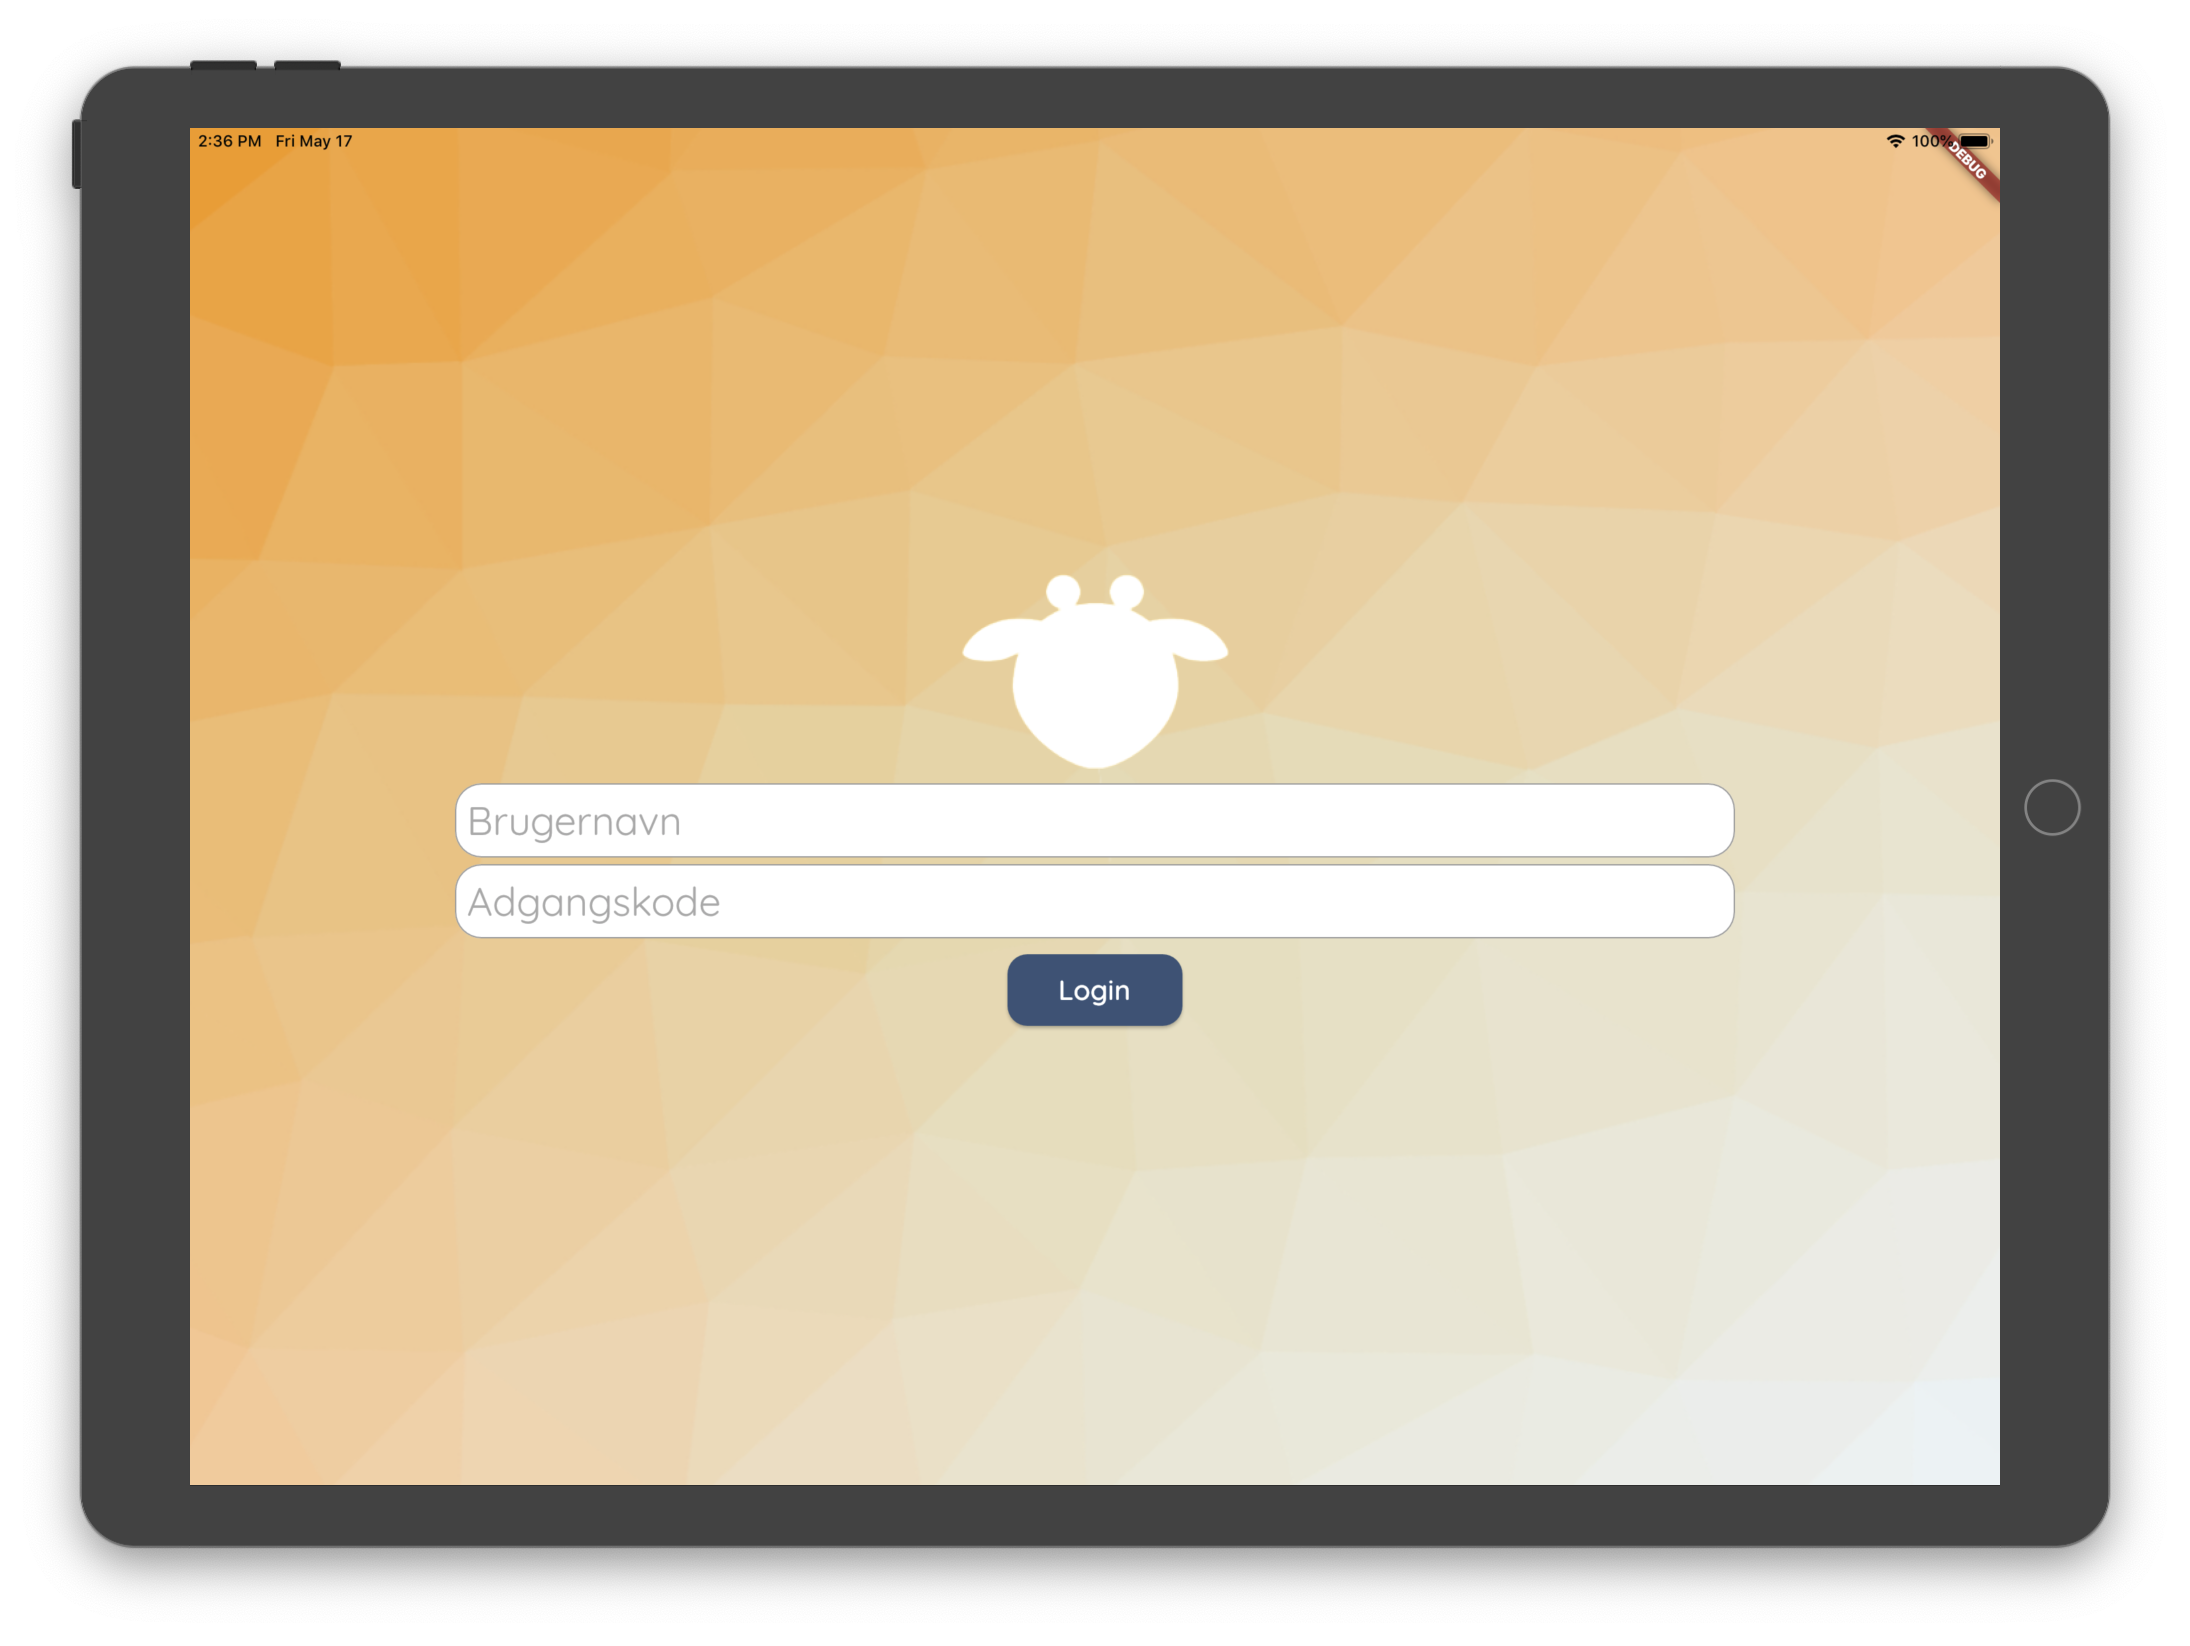
\includegraphics[width=0.95\textwidth]{figures/FinalScreen/loginScreen.png}
    \end{center}
    \caption{Final login screen}
    \label{fig:FinalLoginScreen}
\end{figure}

\subsection{Choose citizen screen}
On the citizen screen you can see an overview of the citizens connected to the user that have logged in, and choose. This shows their names but not pictures. You can either choose a citizen or log out of the application. \ref{fig:finalCitizenScreen} illustrates the screen.
\begin{figure}[H]
    \begin{center}
        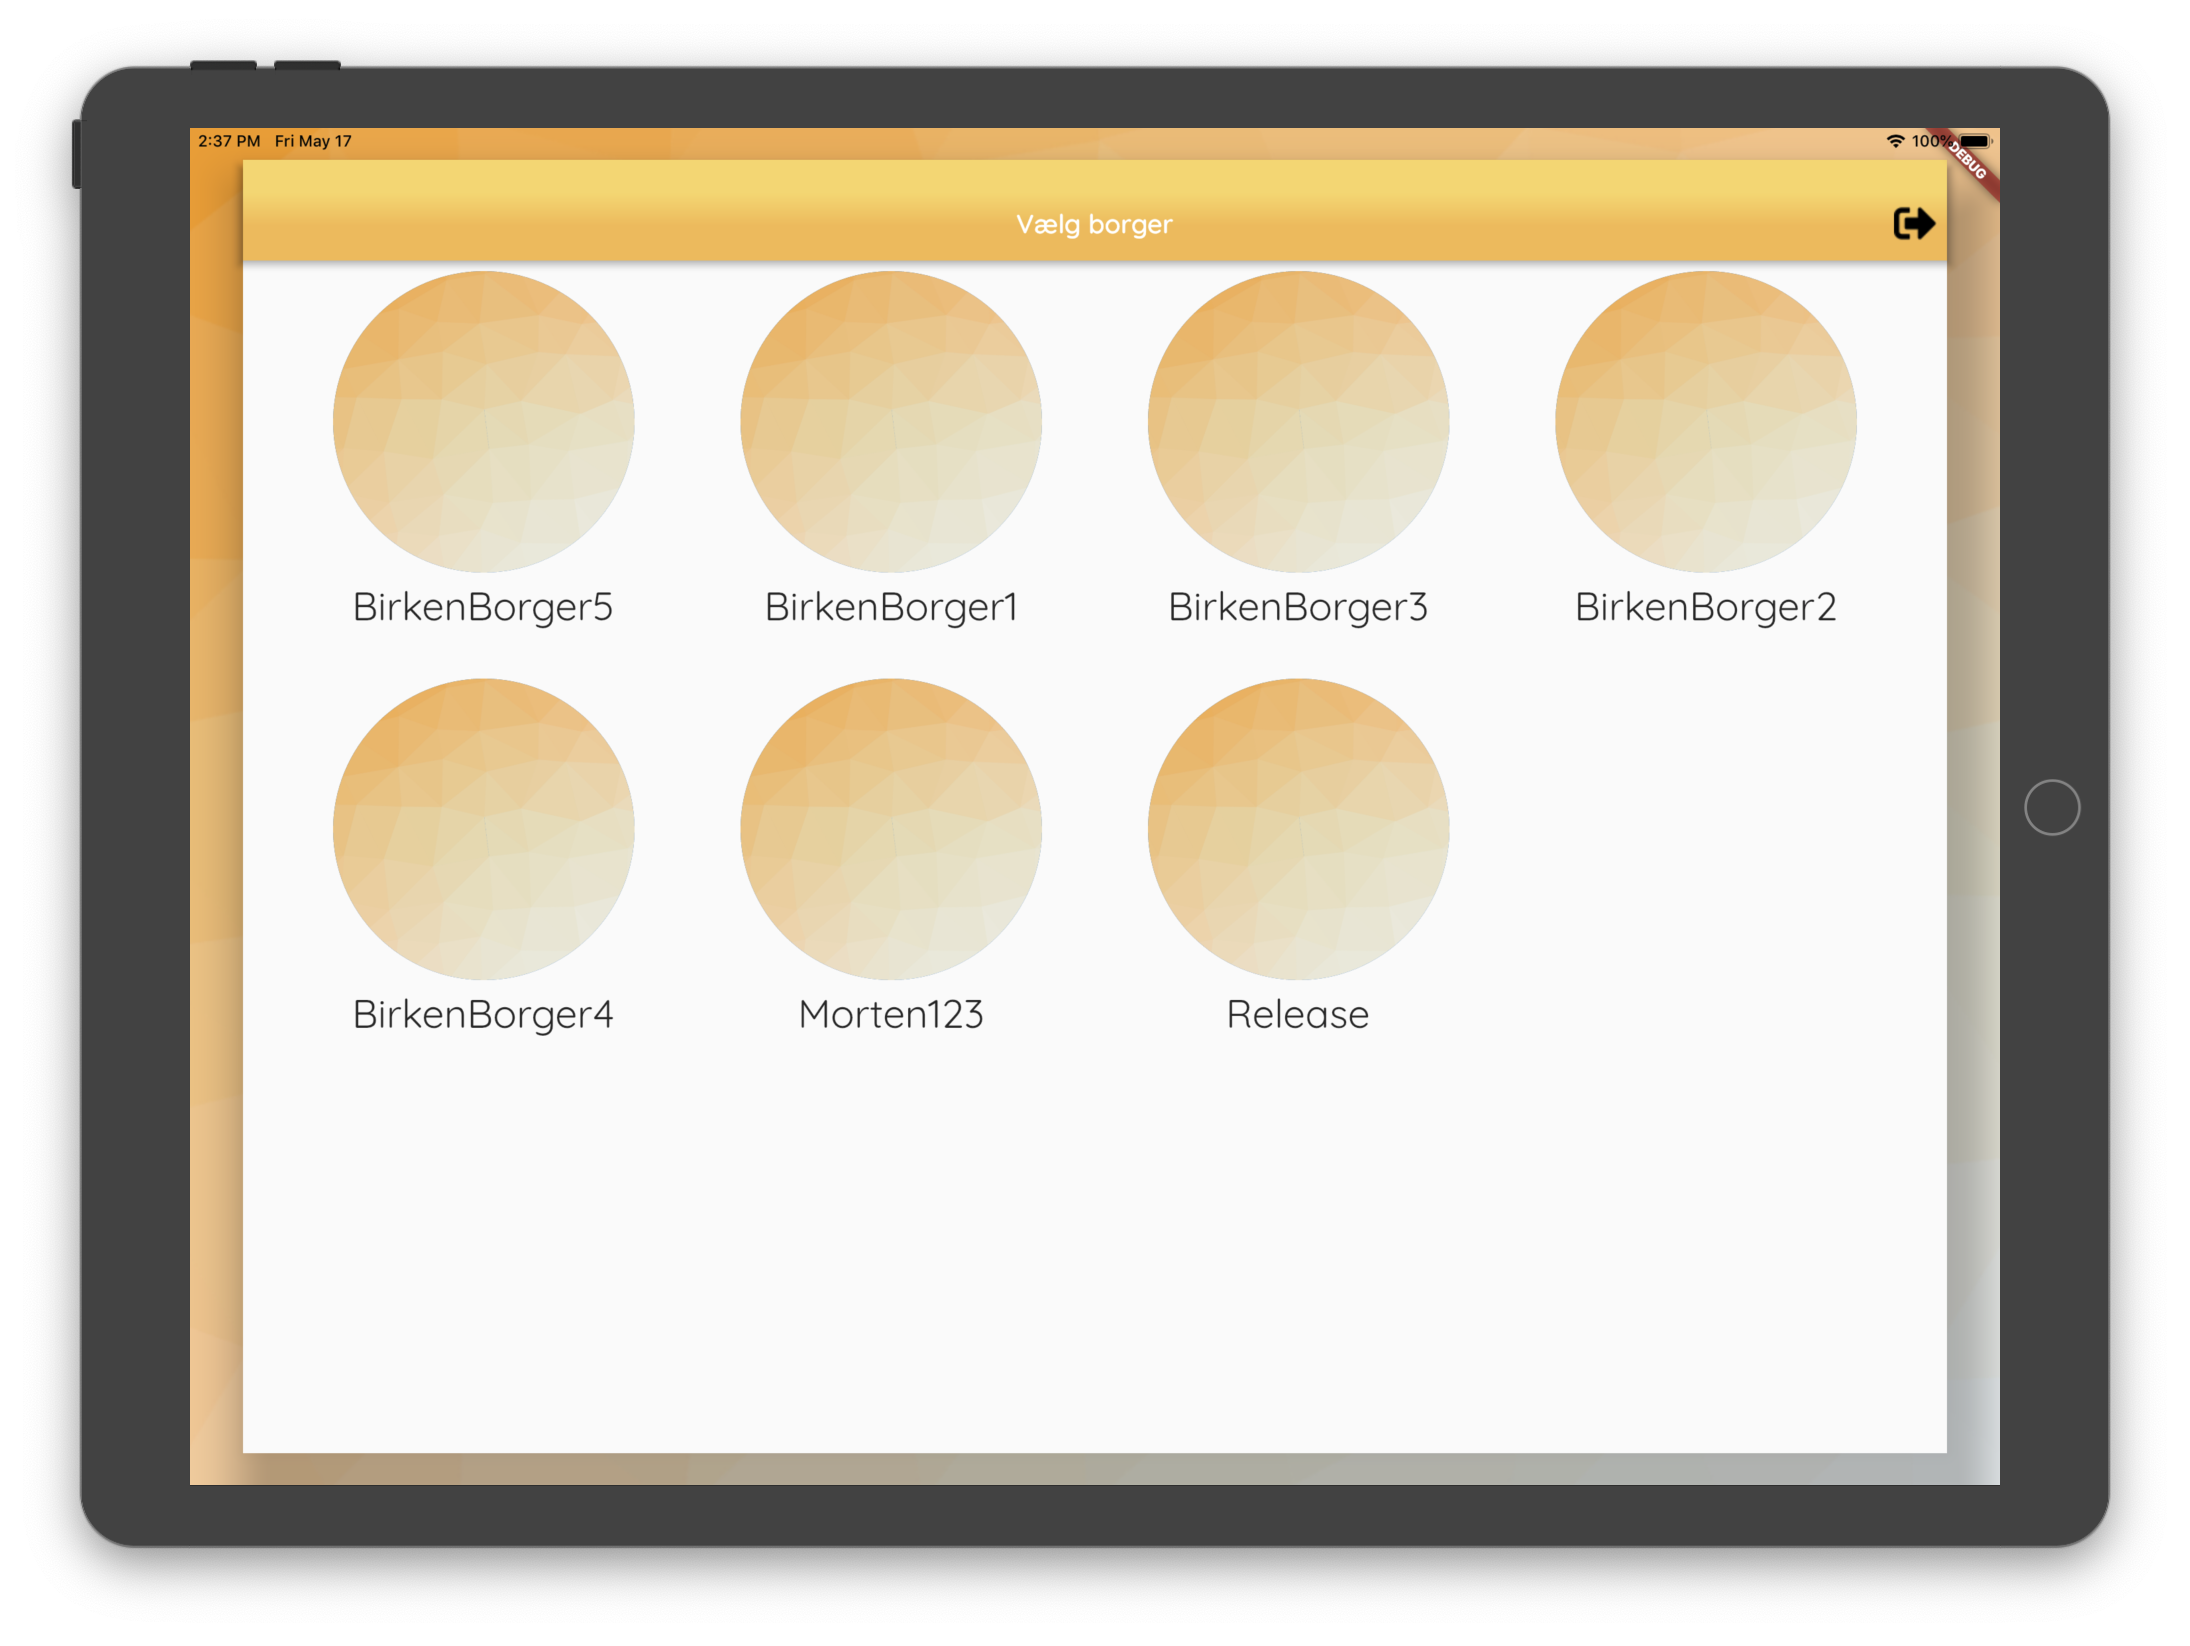
\includegraphics[width=0.95\textwidth]{figures/FinalScreen/chooseCitizenScreen.png}
    \end{center}
    \caption{Final citizen screen}
    \label{fig:finalCitizenScreen}
\end{figure}

\subsection{Weekplan selector screen}
The weekplan selector screen have two modes, a selector mode, shown in \ref{fig:finalCelectWeekplan} and a deletion mode shown in \ref{fig:finalEditWeekplanSelector}.

\begin{figure}[H]
    \begin{center}
        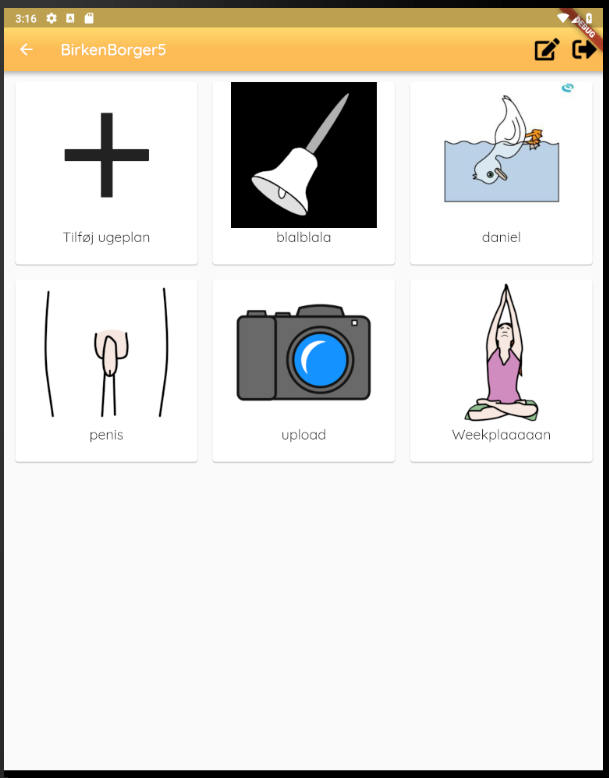
\includegraphics[width=0.95\textwidth]{figures/FinalScreen/chooseWeekplanScreen.png}
    \end{center}
    \caption{Final citizen screen}
    \label{fig:finalCelectWeekplan}
\end{figure}

\begin{figure}[H]
    \begin{center}
        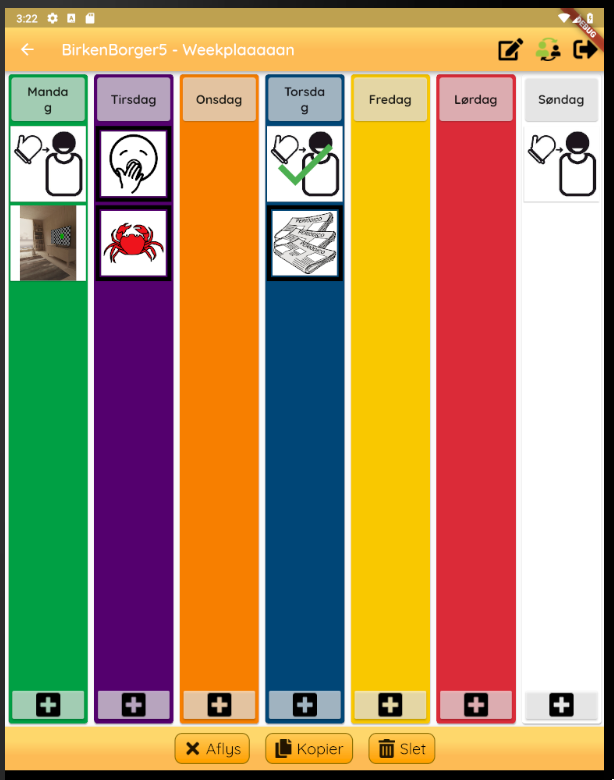
\includegraphics[width=0.95\textwidth]{figures/FinalScreen/editWeekplanScreen.png}
    \end{center}
    \caption{Final citizen screen}
    \label{fig:finalEditWeekplanSelector}
\end{figure}

In the selector mode you can either create a new weekplan or choose a weekplan. In the deletion mode you can delete a variable number of weekplans. The weekplans marked with black in \ref{fig:finalEditWeekplanSelector} are chosen for deletion. The add weekplan button are still present in this mode, but does not do anything. 

\subsection{New weekplan screen}

The add weekplan screen is shown in \ref{fig:finalAddWeekplanSelector}.
\begin{figure}[H]
    \begin{center}
        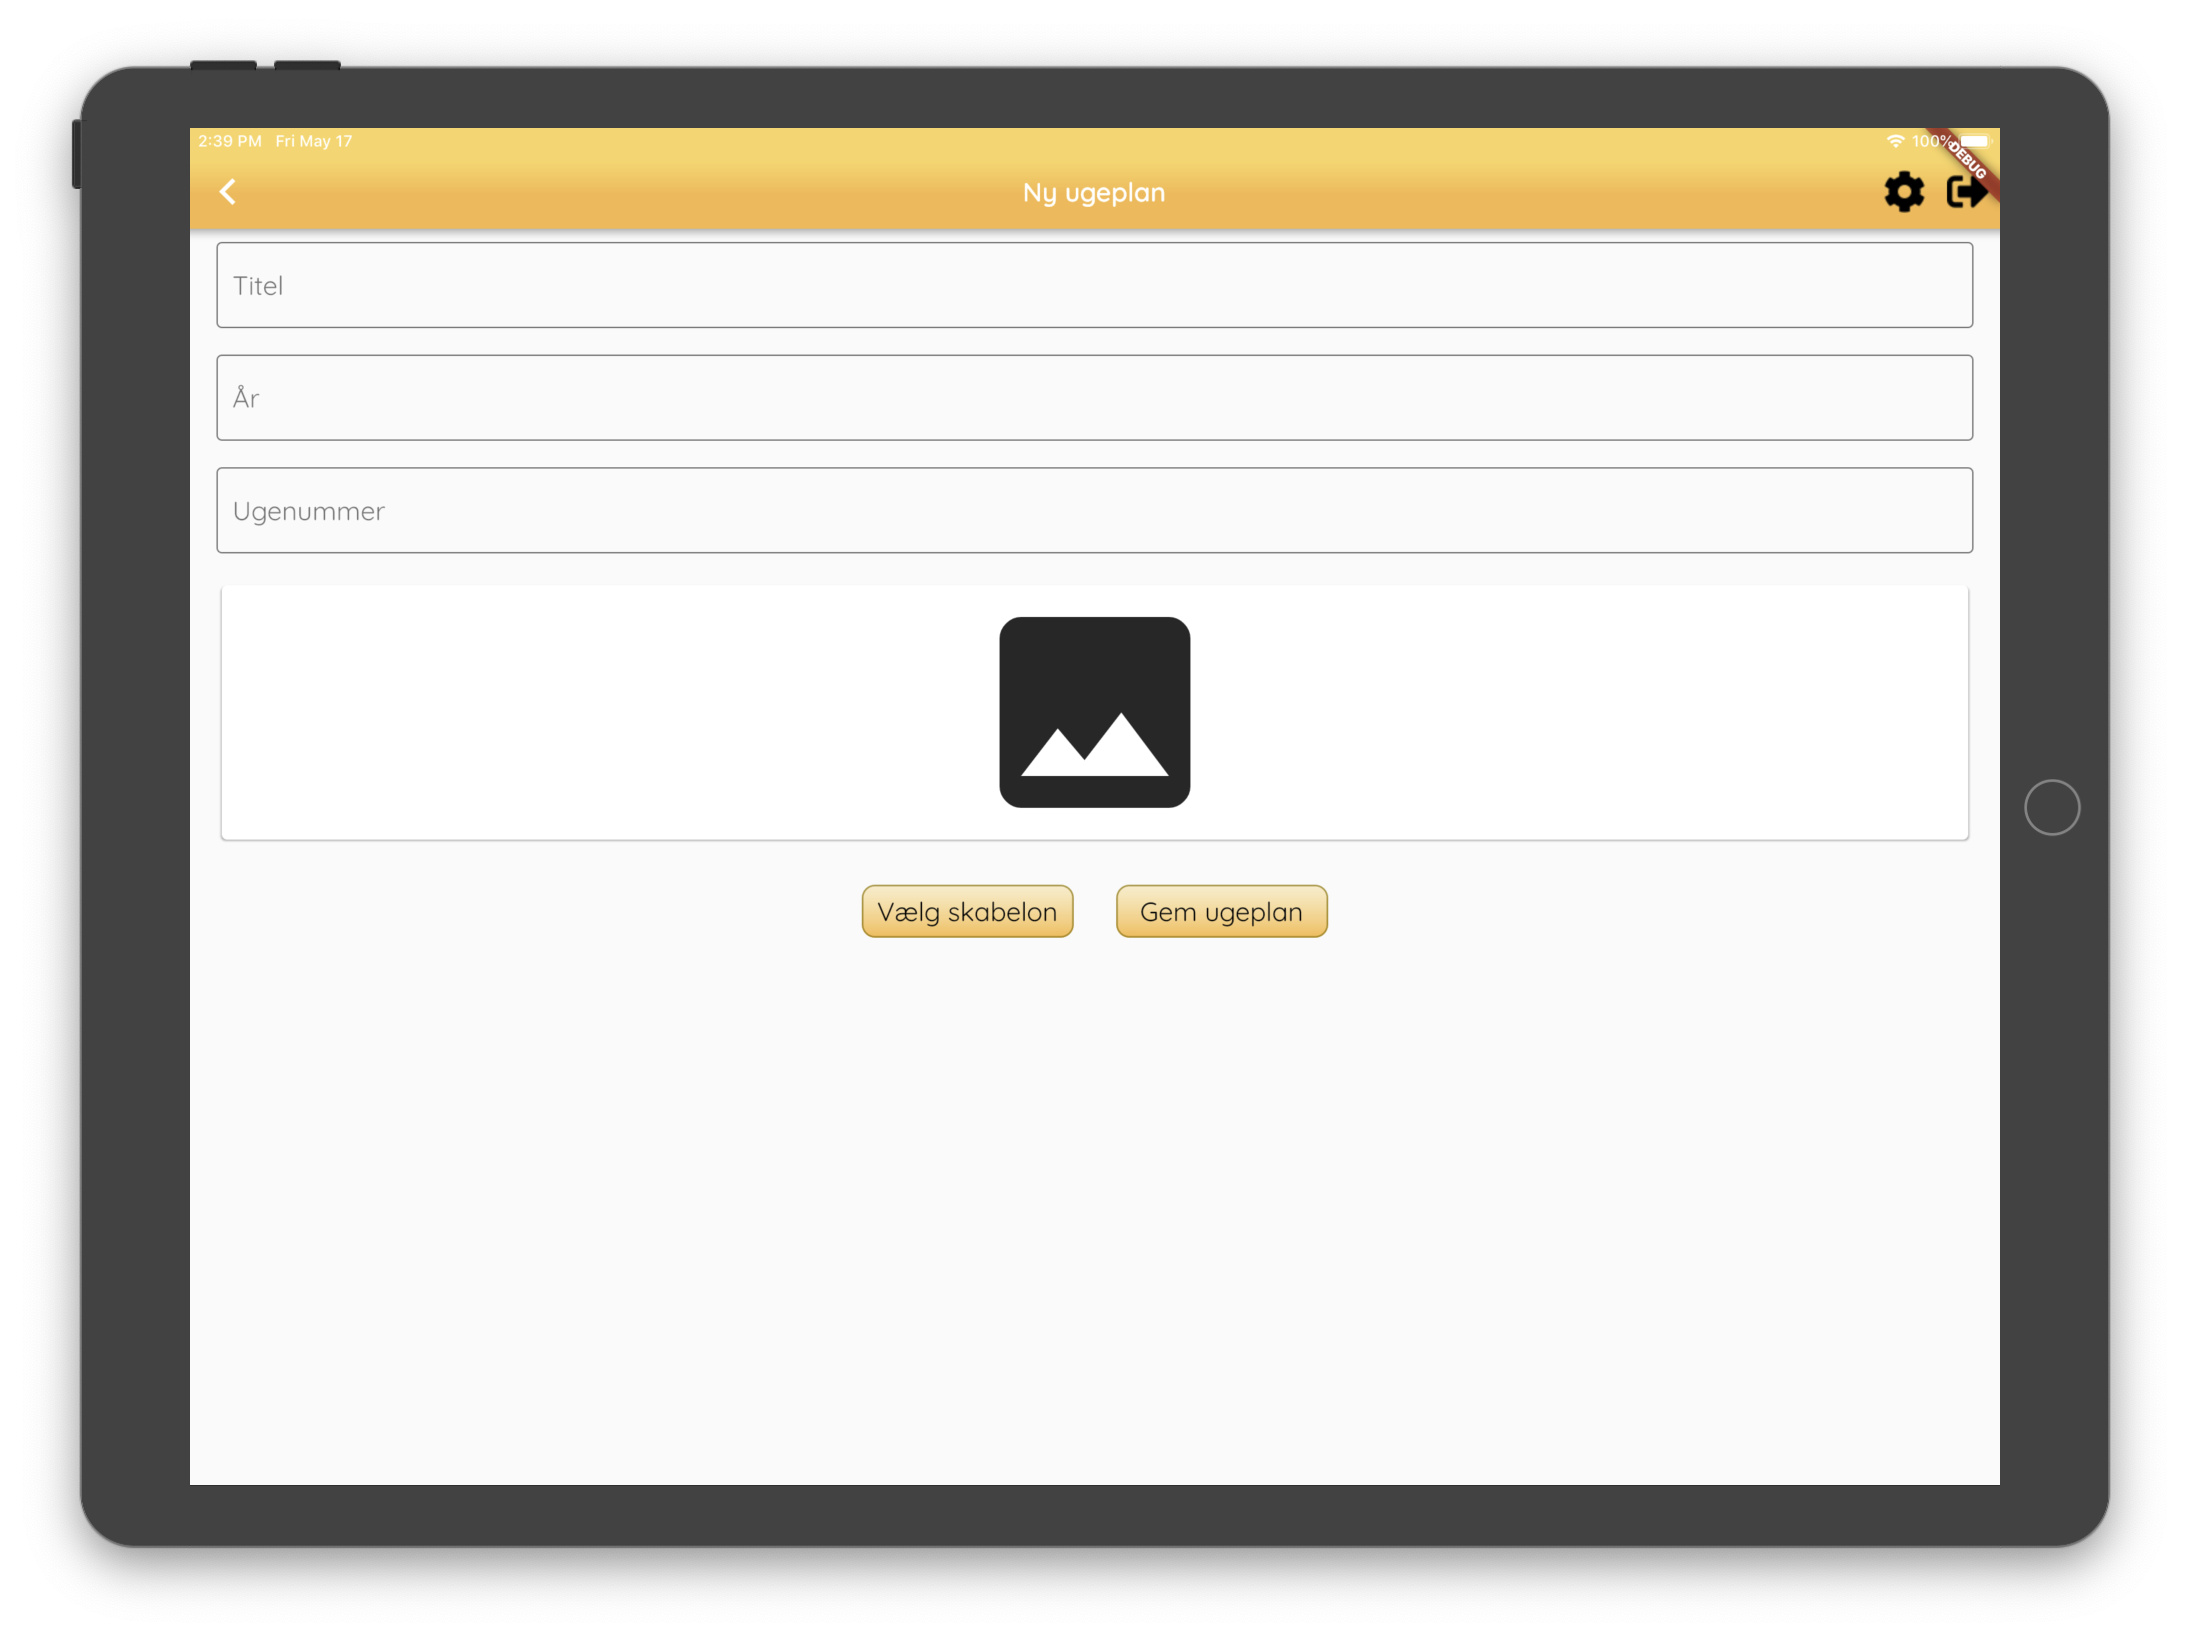
\includegraphics[width=0.95\textwidth]{figures/FinalScreen/addWeekplanScreen.png}
    \end{center}
    \caption{Final new weekplan screen}
    \label{fig:finalAddWeekplanSelector}
\end{figure}
Here you can enter a title, year, week number and picture, and make a new weekplan. If you tab the picture field you will be redirected to the pictogram seach screen, where you can choose a picture for the weekplan. 

\subsection{Weekplan screen}
The weekplan screen has three modes, guardian mode, , edit mode and citizen mode. 
\begin{figure}[H]
    \begin{center}
        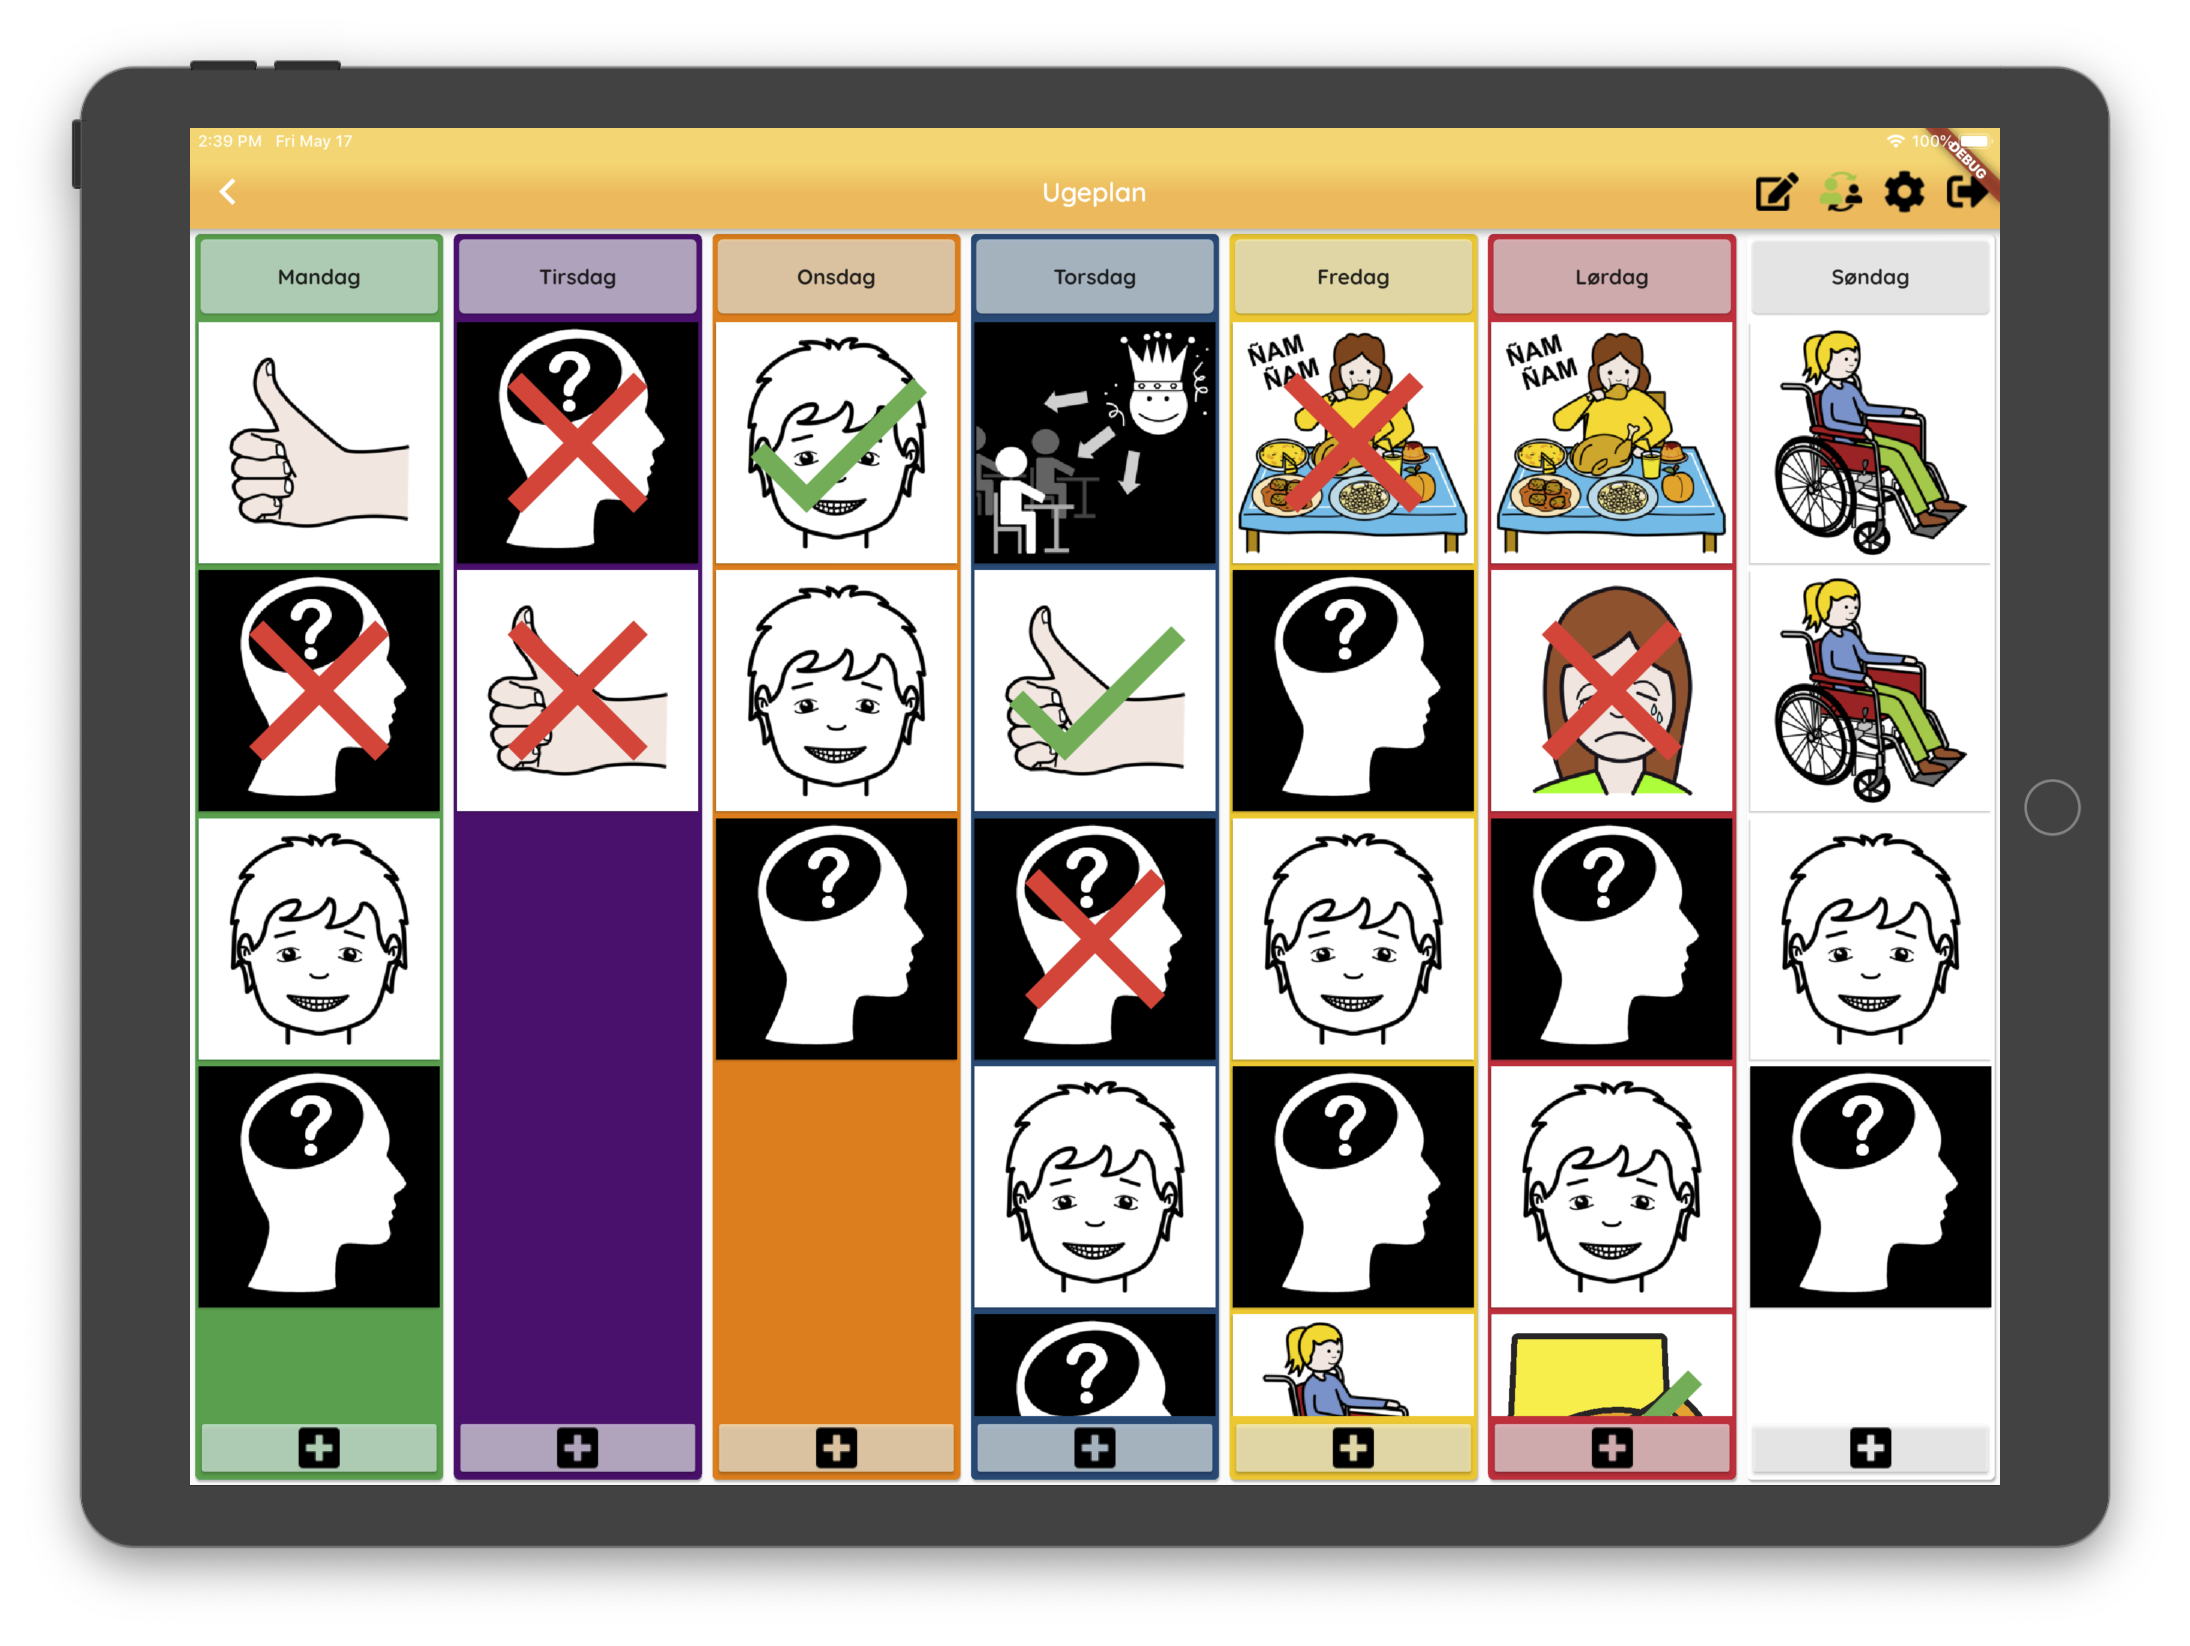
\includegraphics[width=0.95\textwidth]{figures/FinalScreen/weekplanScreen.png}
    \end{center}
    \caption{Final weekplan screen in guardian mode}
    \label{fig:finalWeekplanGuardianMode}
\end{figure}
\begin{figure}[H]
    \begin{center}
        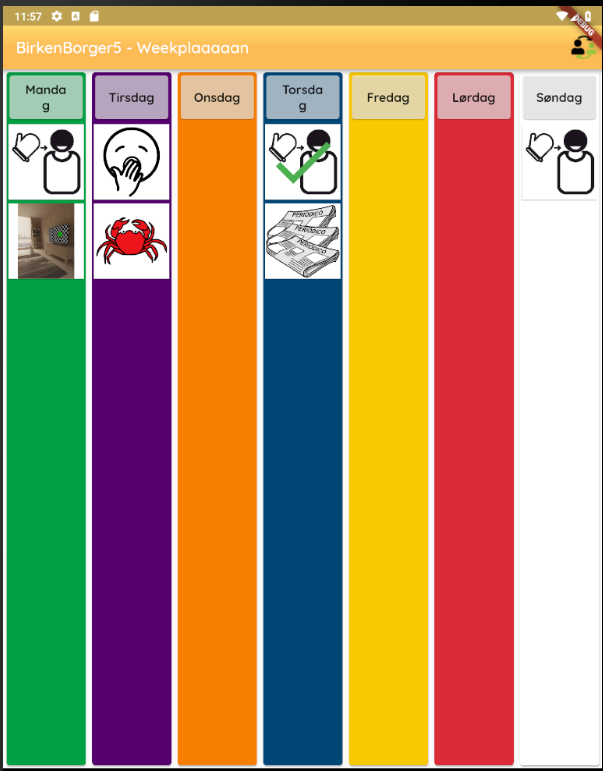
\includegraphics[width=0.95\textwidth]{figures/FinalScreen/weekplanScreenMoveActivity.png}
    \end{center}
    \caption{Move an activity in a weekplan}
    \label{fig:finalWeekplanMoveActivity}
\end{figure}

\begin{figure}[H]
    \begin{center}
        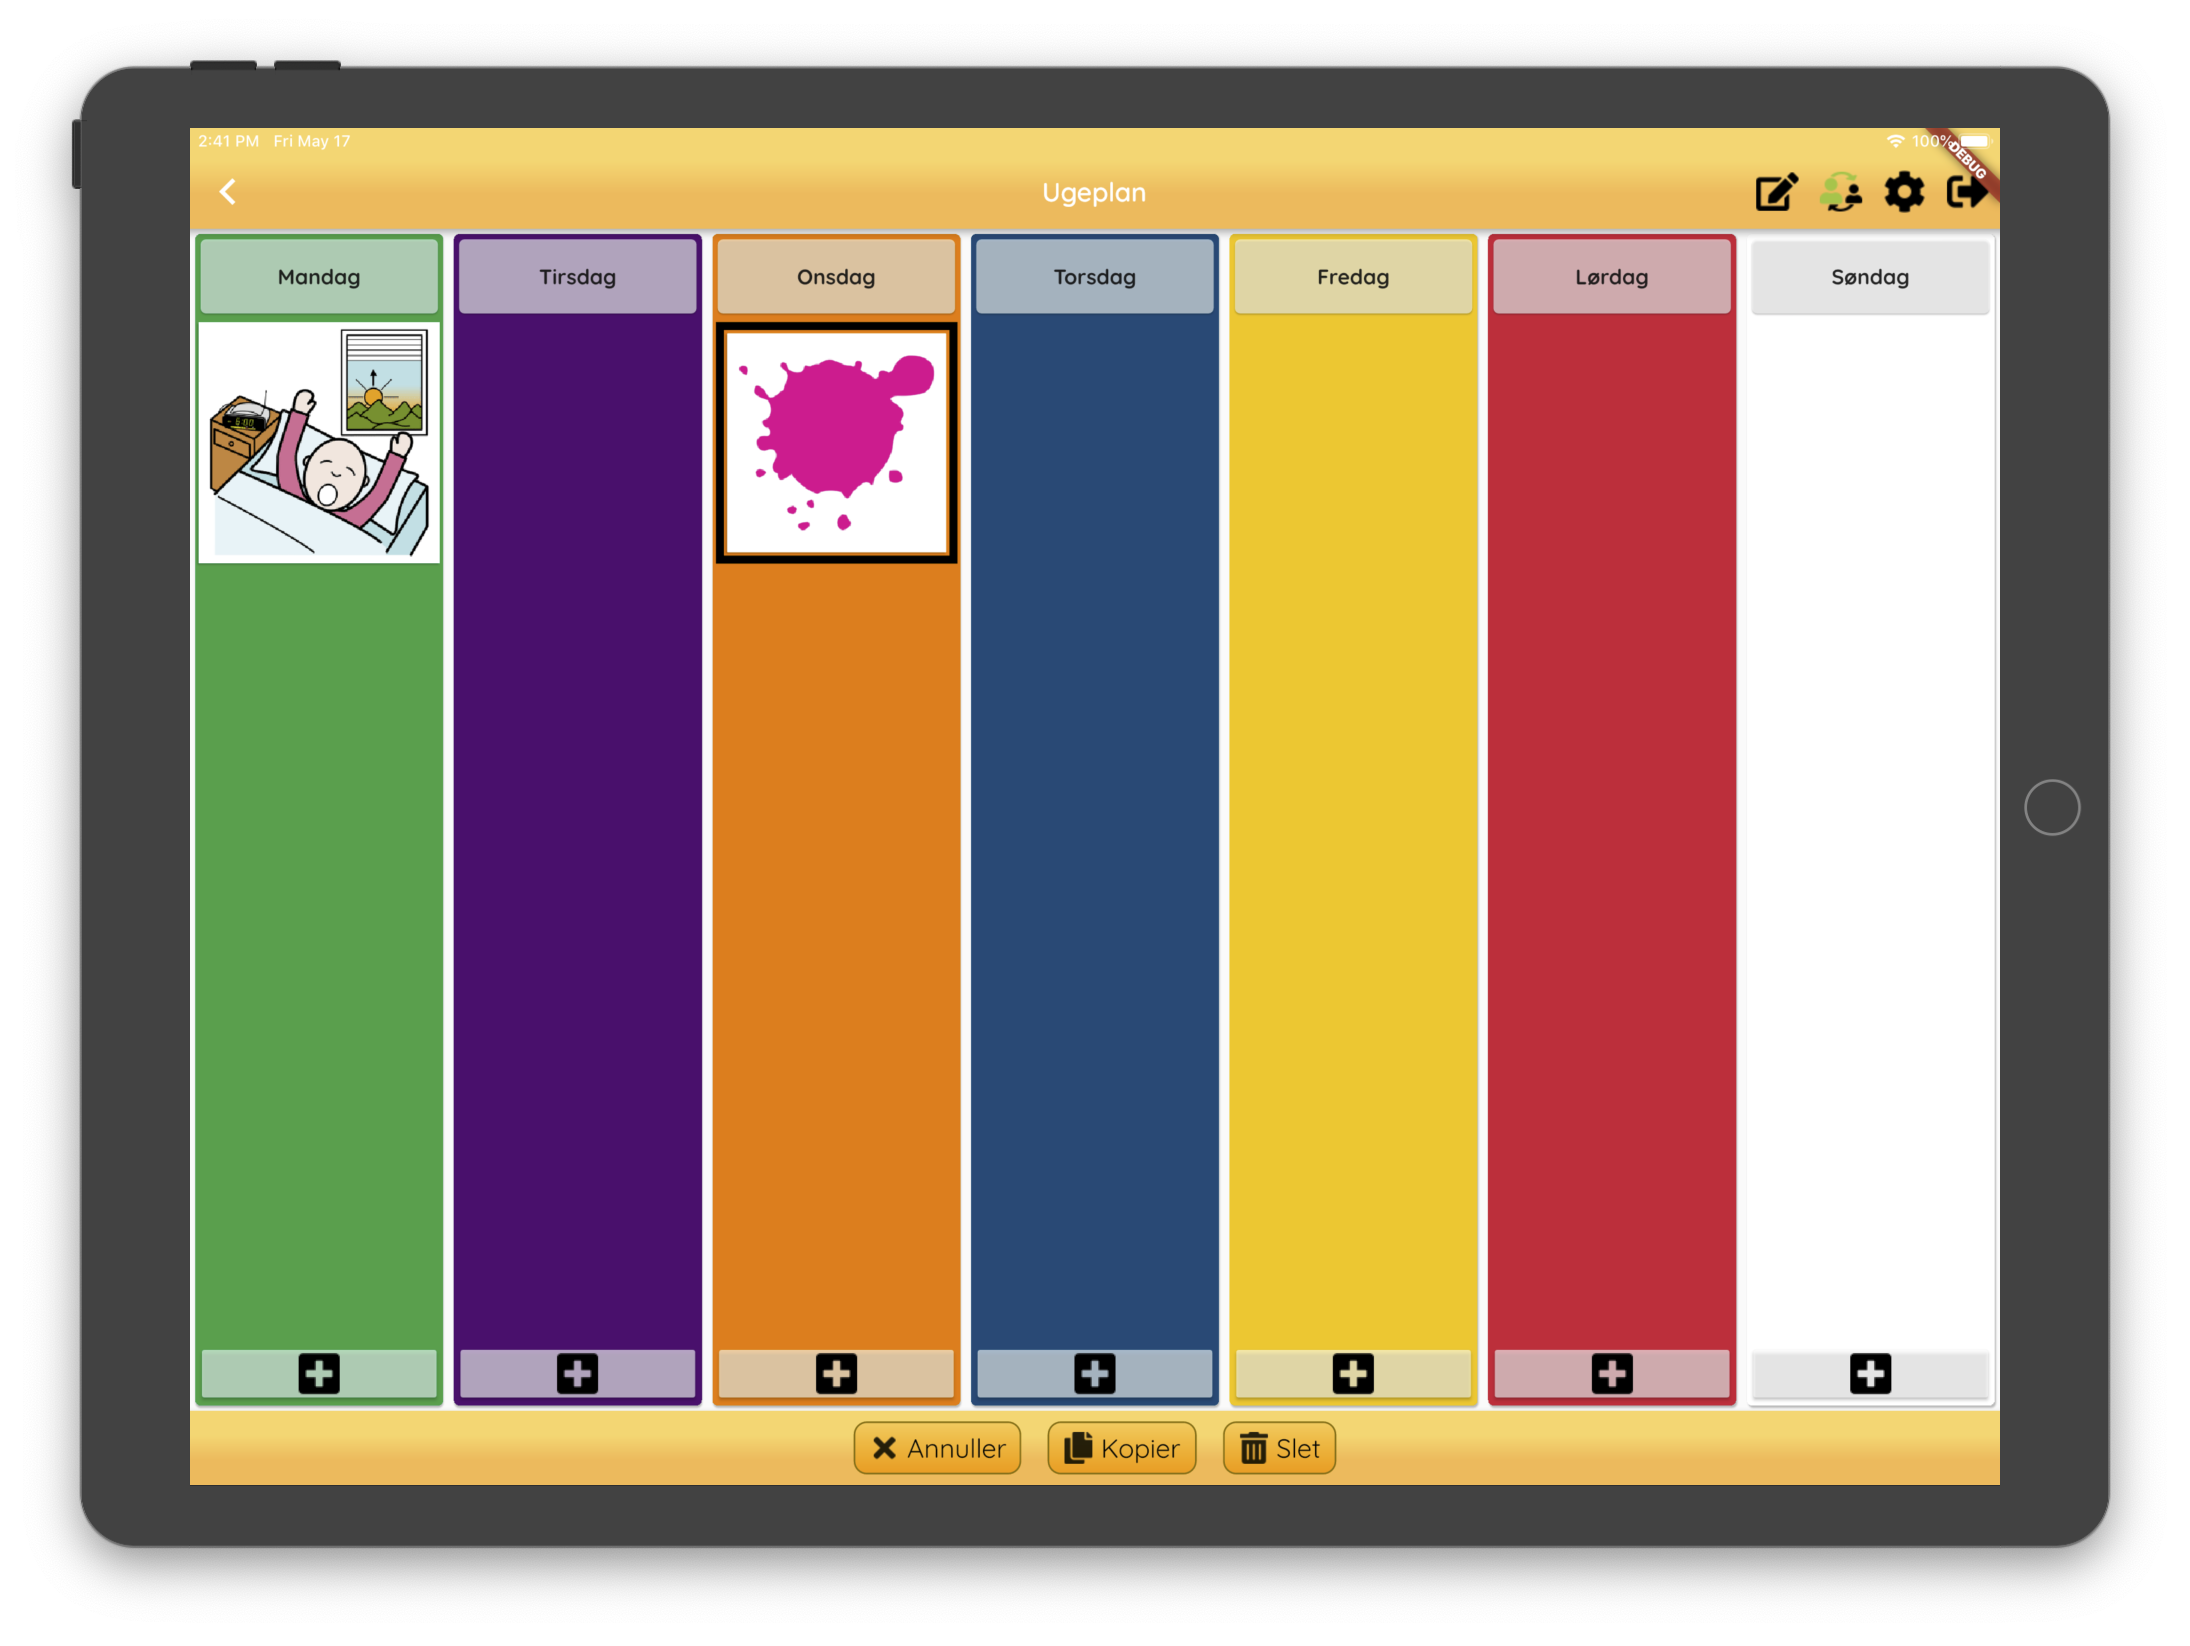
\includegraphics[width=0.95\textwidth]{figures/FinalScreen/editWeekplanScreenMarked.png}
    \end{center}
    \caption{A weekplan screen in edit mode with two activities marked}
    \label{fig:finalWeekplanEditMode}
\end{figure}
\begin{figure}[H]
    \begin{center}
        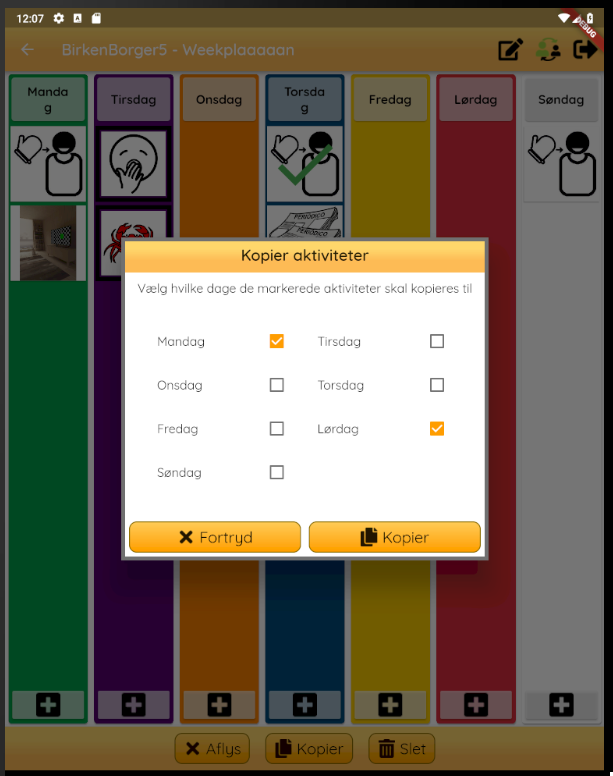
\includegraphics[width=0.95\textwidth]{figures/FinalScreen/editWeekplanScreenCopy.png}
    \end{center}
    \caption{The copy pop up to select days to copy to}
    \label{fig:finalWeekplanScreenCopy}
\end{figure}
\begin{figure}[H]
    \begin{center}
        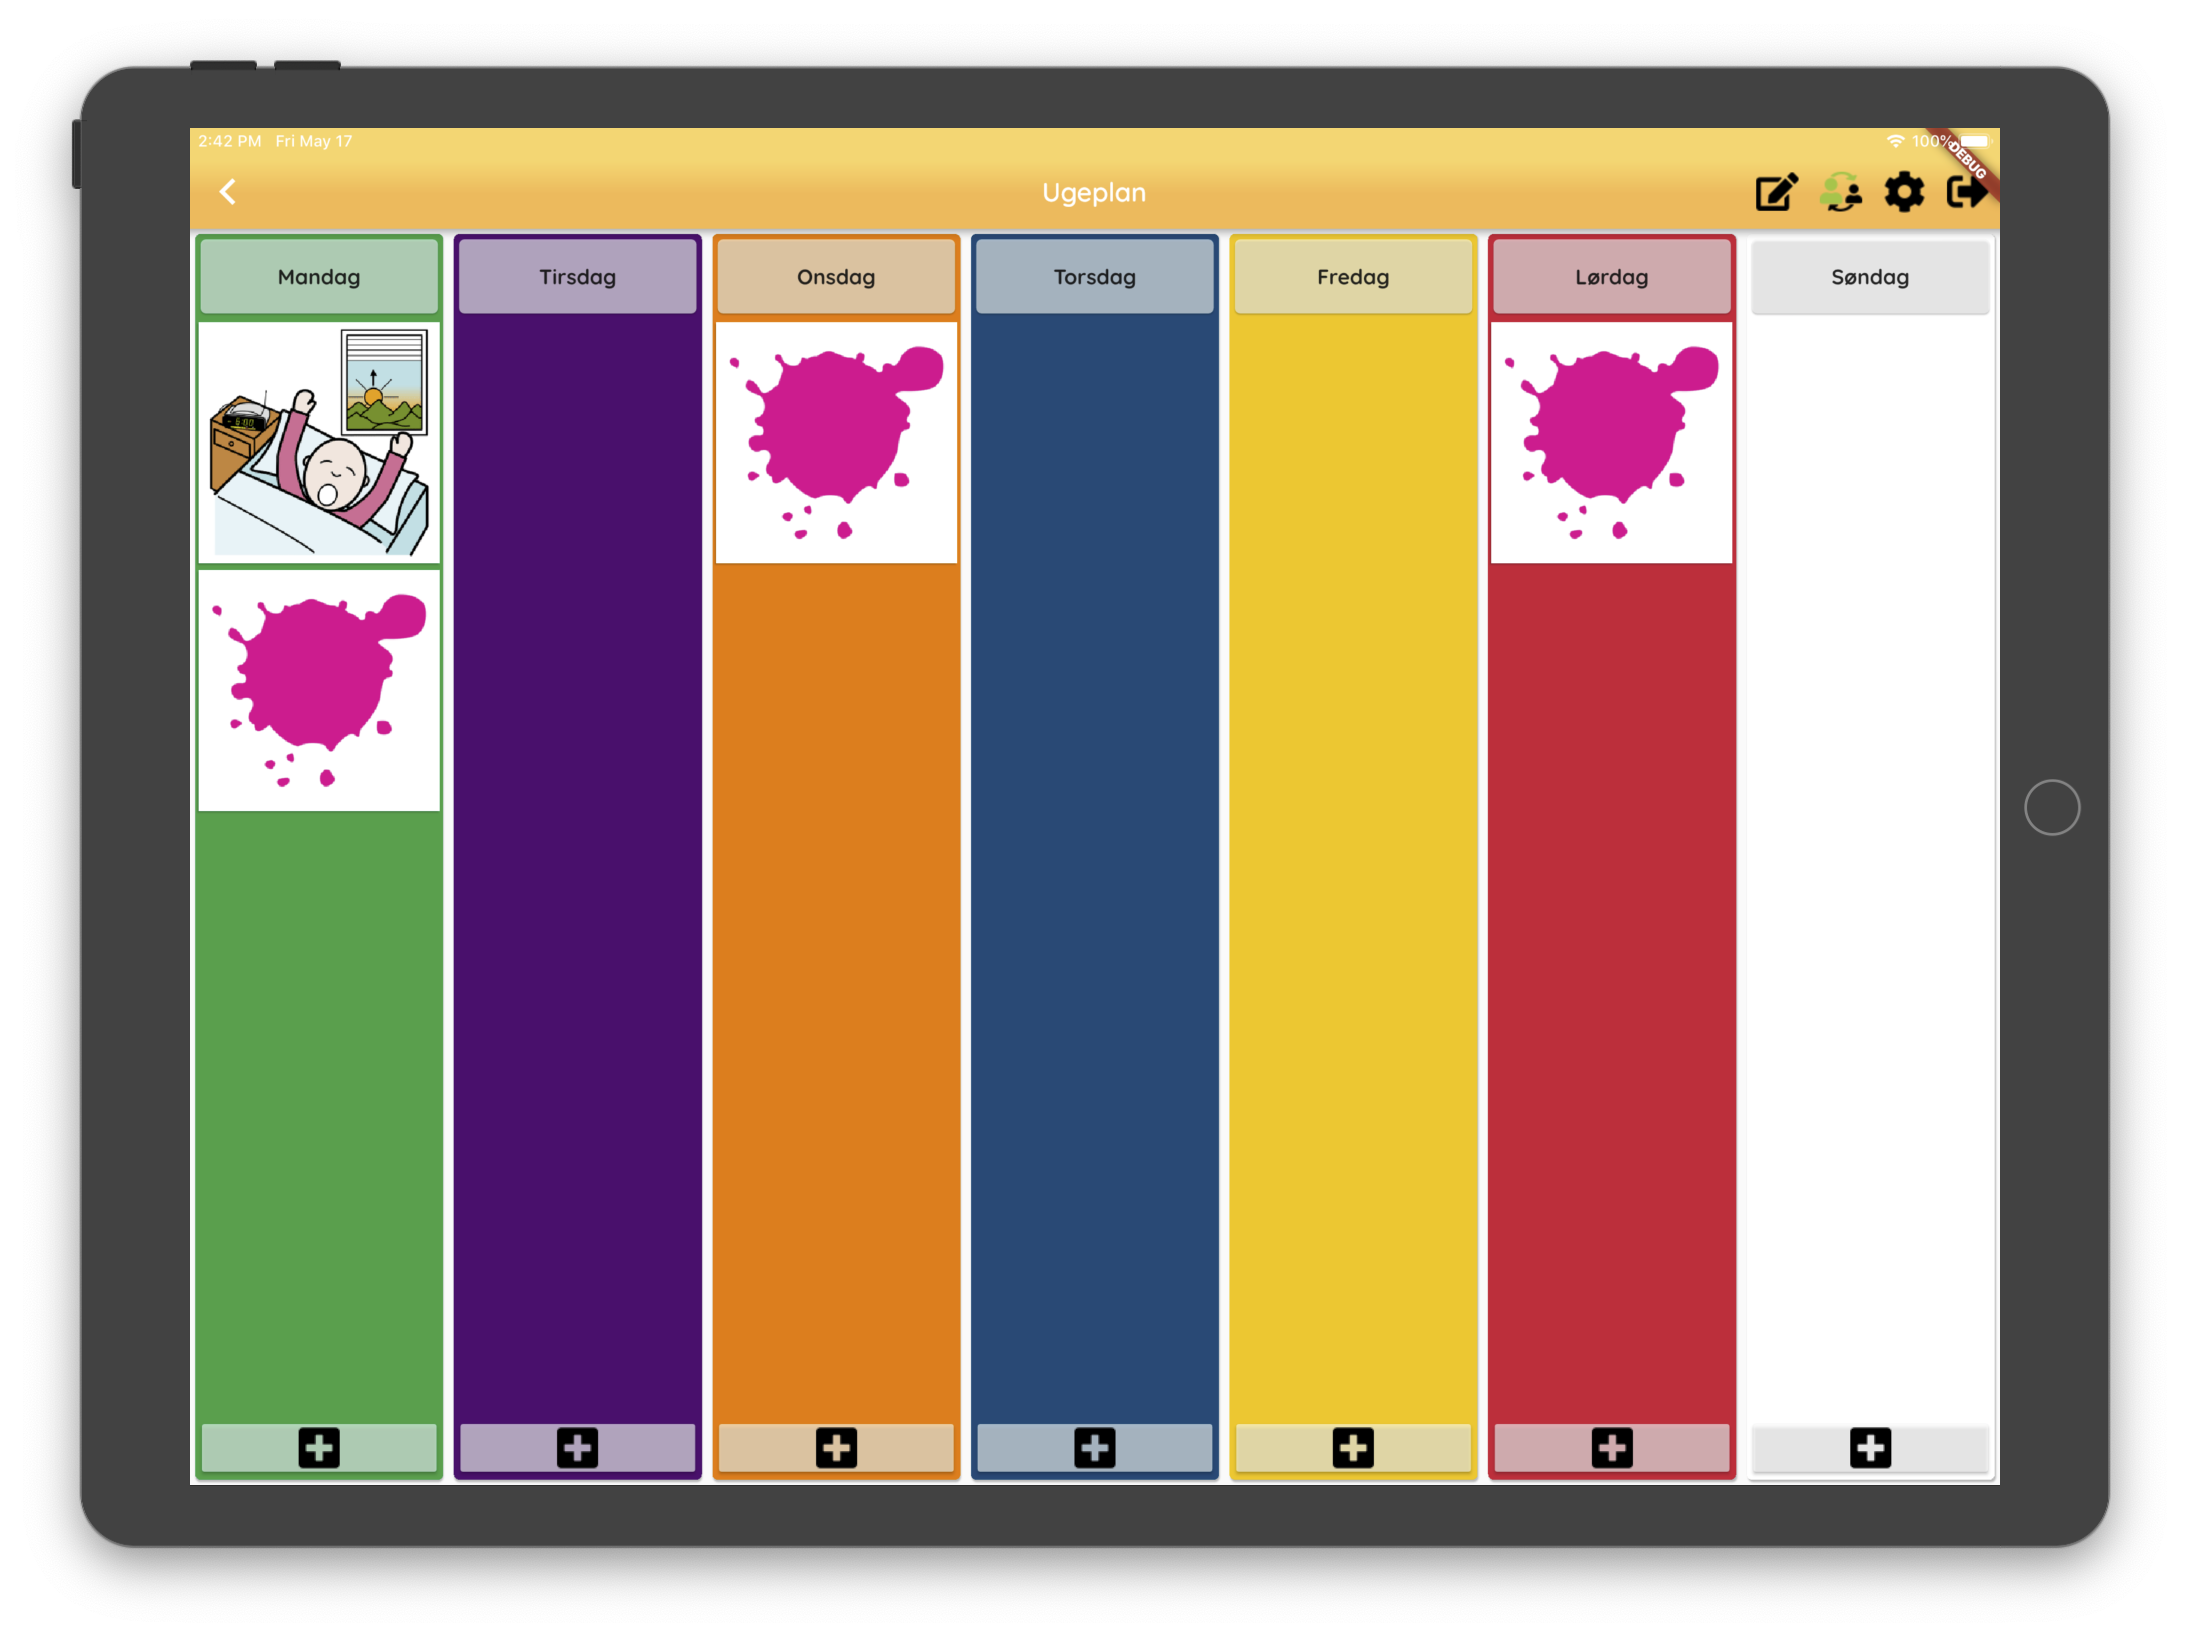
\includegraphics[width=0.95\textwidth]{figures/FinalScreen/editWeekplanScreenAfterCopy.png}
    \end{center}
    \caption{The weekplan after content have been copied}
    \label{fig:finalWeekplanAfterCopy}
\end{figure}

\begin{figure}[H]
    \begin{center}
        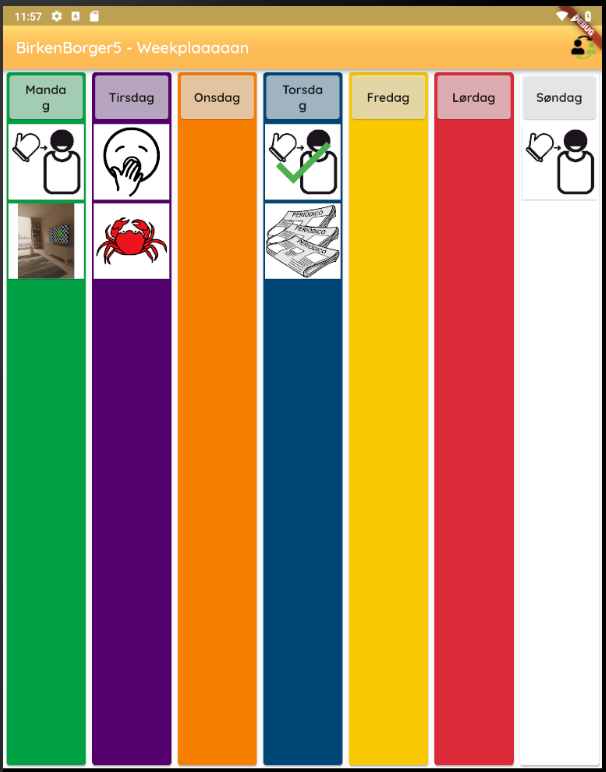
\includegraphics[width=0.95\textwidth]{figures/FinalScreen/weekplanScreenCitizenMode.png}
    \end{center}
    \caption{Final weekplan screen when in citizen mode}
    \label{fig:finalWeekplanCitizenMode}
\end{figure}

When the weekplan screen are in guardian mode it is possible to change to citizen or edit mode, enter activities or move activities as in \ref{fig:finalWeekplanMoveActivity}. When you move an activity you have to hold it a few seconds and then move it to the desired location. It will be placed before the field where you let go.

In edit mode you can either switch to the other modes, or edit the weekplan. You can mark a variable number of activities, and either delete them or copy them to any number of days. \ref{fig:finalWeekplanEditMode} shows two selected pictograms. If you want to copy them you click on copy and a popup appears, seen in \ref{fig:finalWeekplanScreenCopy}. The pictograms will then be placed in the end of the chosen days as in \ref{fig:finalWeekplanAfterCopy}. 

In citizen mode there are less functionalities. The citizen can not go back to the select screen, log out or edit in any way. The only things a citizen can do is open a show activity screen or change to guardian. 

When a user tries to switch from citizen to guardian mode he has to enter a password, while he only has to confirm the other way round. 

\subsection{Pictogram search screen}
The pictogram search screen is shown in \ref{fig:finalPictogramSeach}.

\begin{figure}[H]
    \begin{center}
        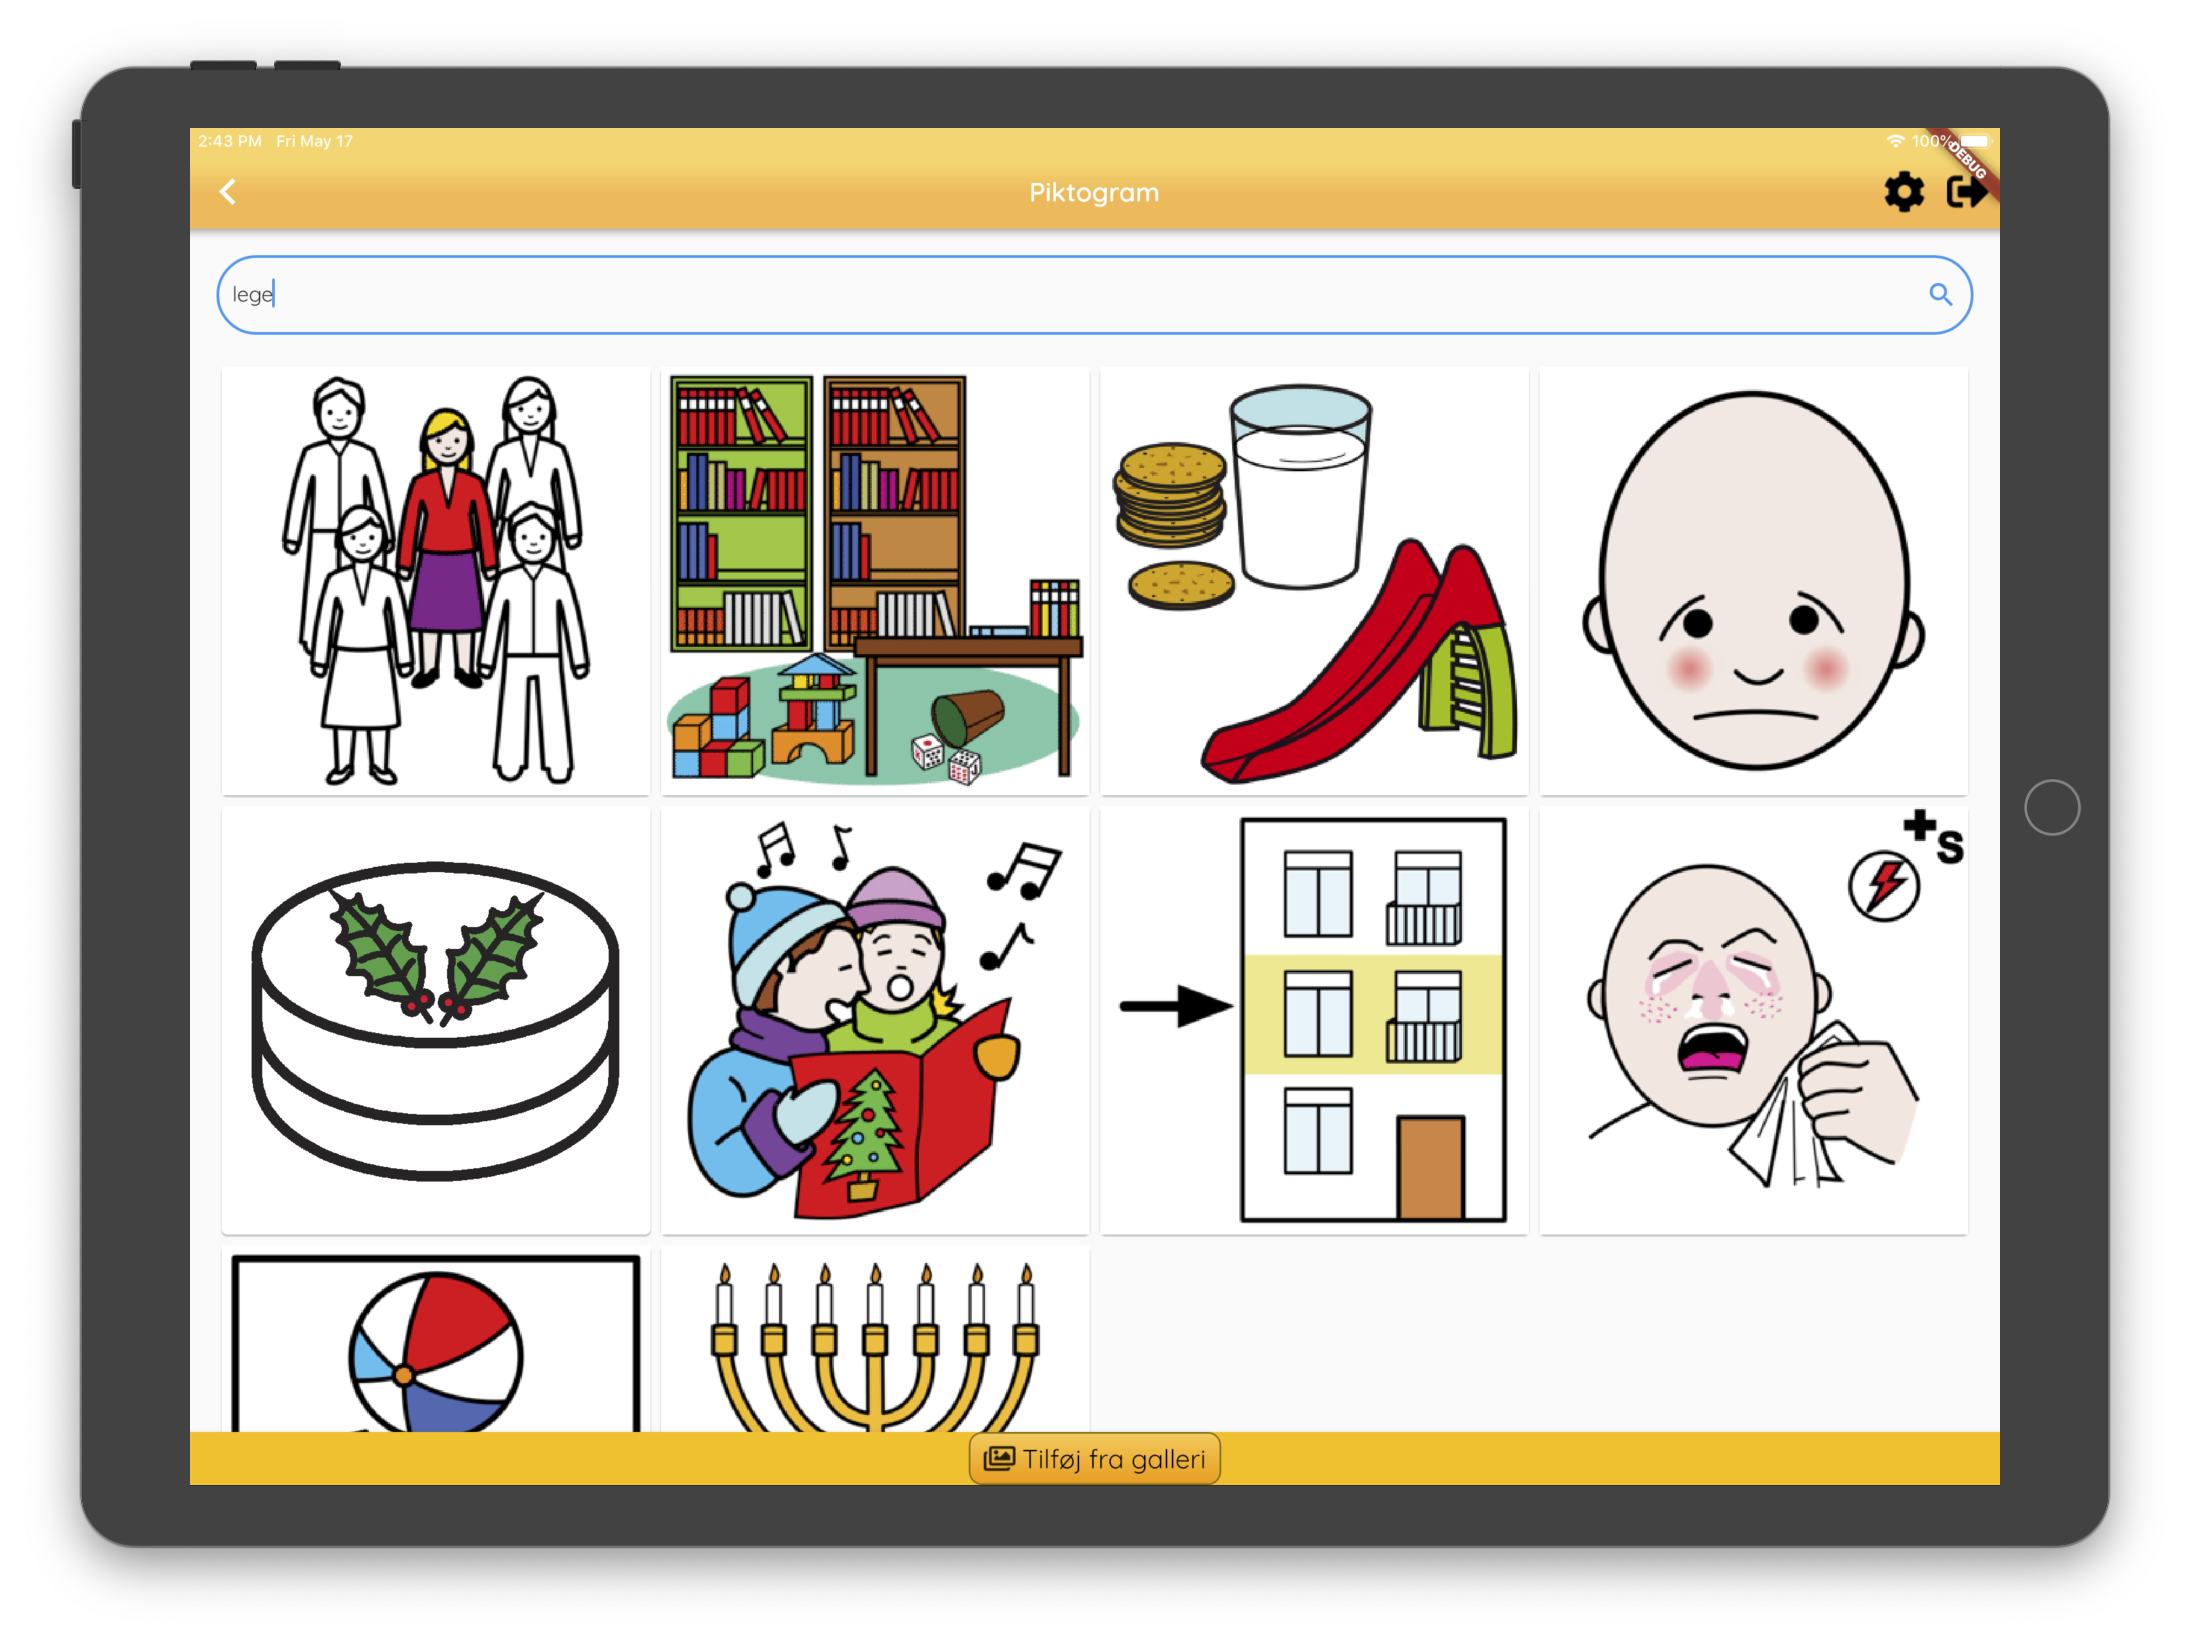
\includegraphics[width=0.95\textwidth]{figures/FinalScreen/addPictogramScreen.png}
    \end{center}
    \caption{Screen to search for pictograms}
    \label{fig:finalPictogramSeach}
\end{figure}

The Pictogram seach screen can show pictures from the database. When text is entered in the text field, the screen shows ten pictures with a name that contains the text. The application navigates to thee Upload image from phone screen when the button in the bottom are clicked.

\subsection{Show activity screen}
The Show activity screen looks different if the app is in citizen mode than it does in guardian mode.
In citizen mode. 

\begin{figure}[H]
    \begin{center}
        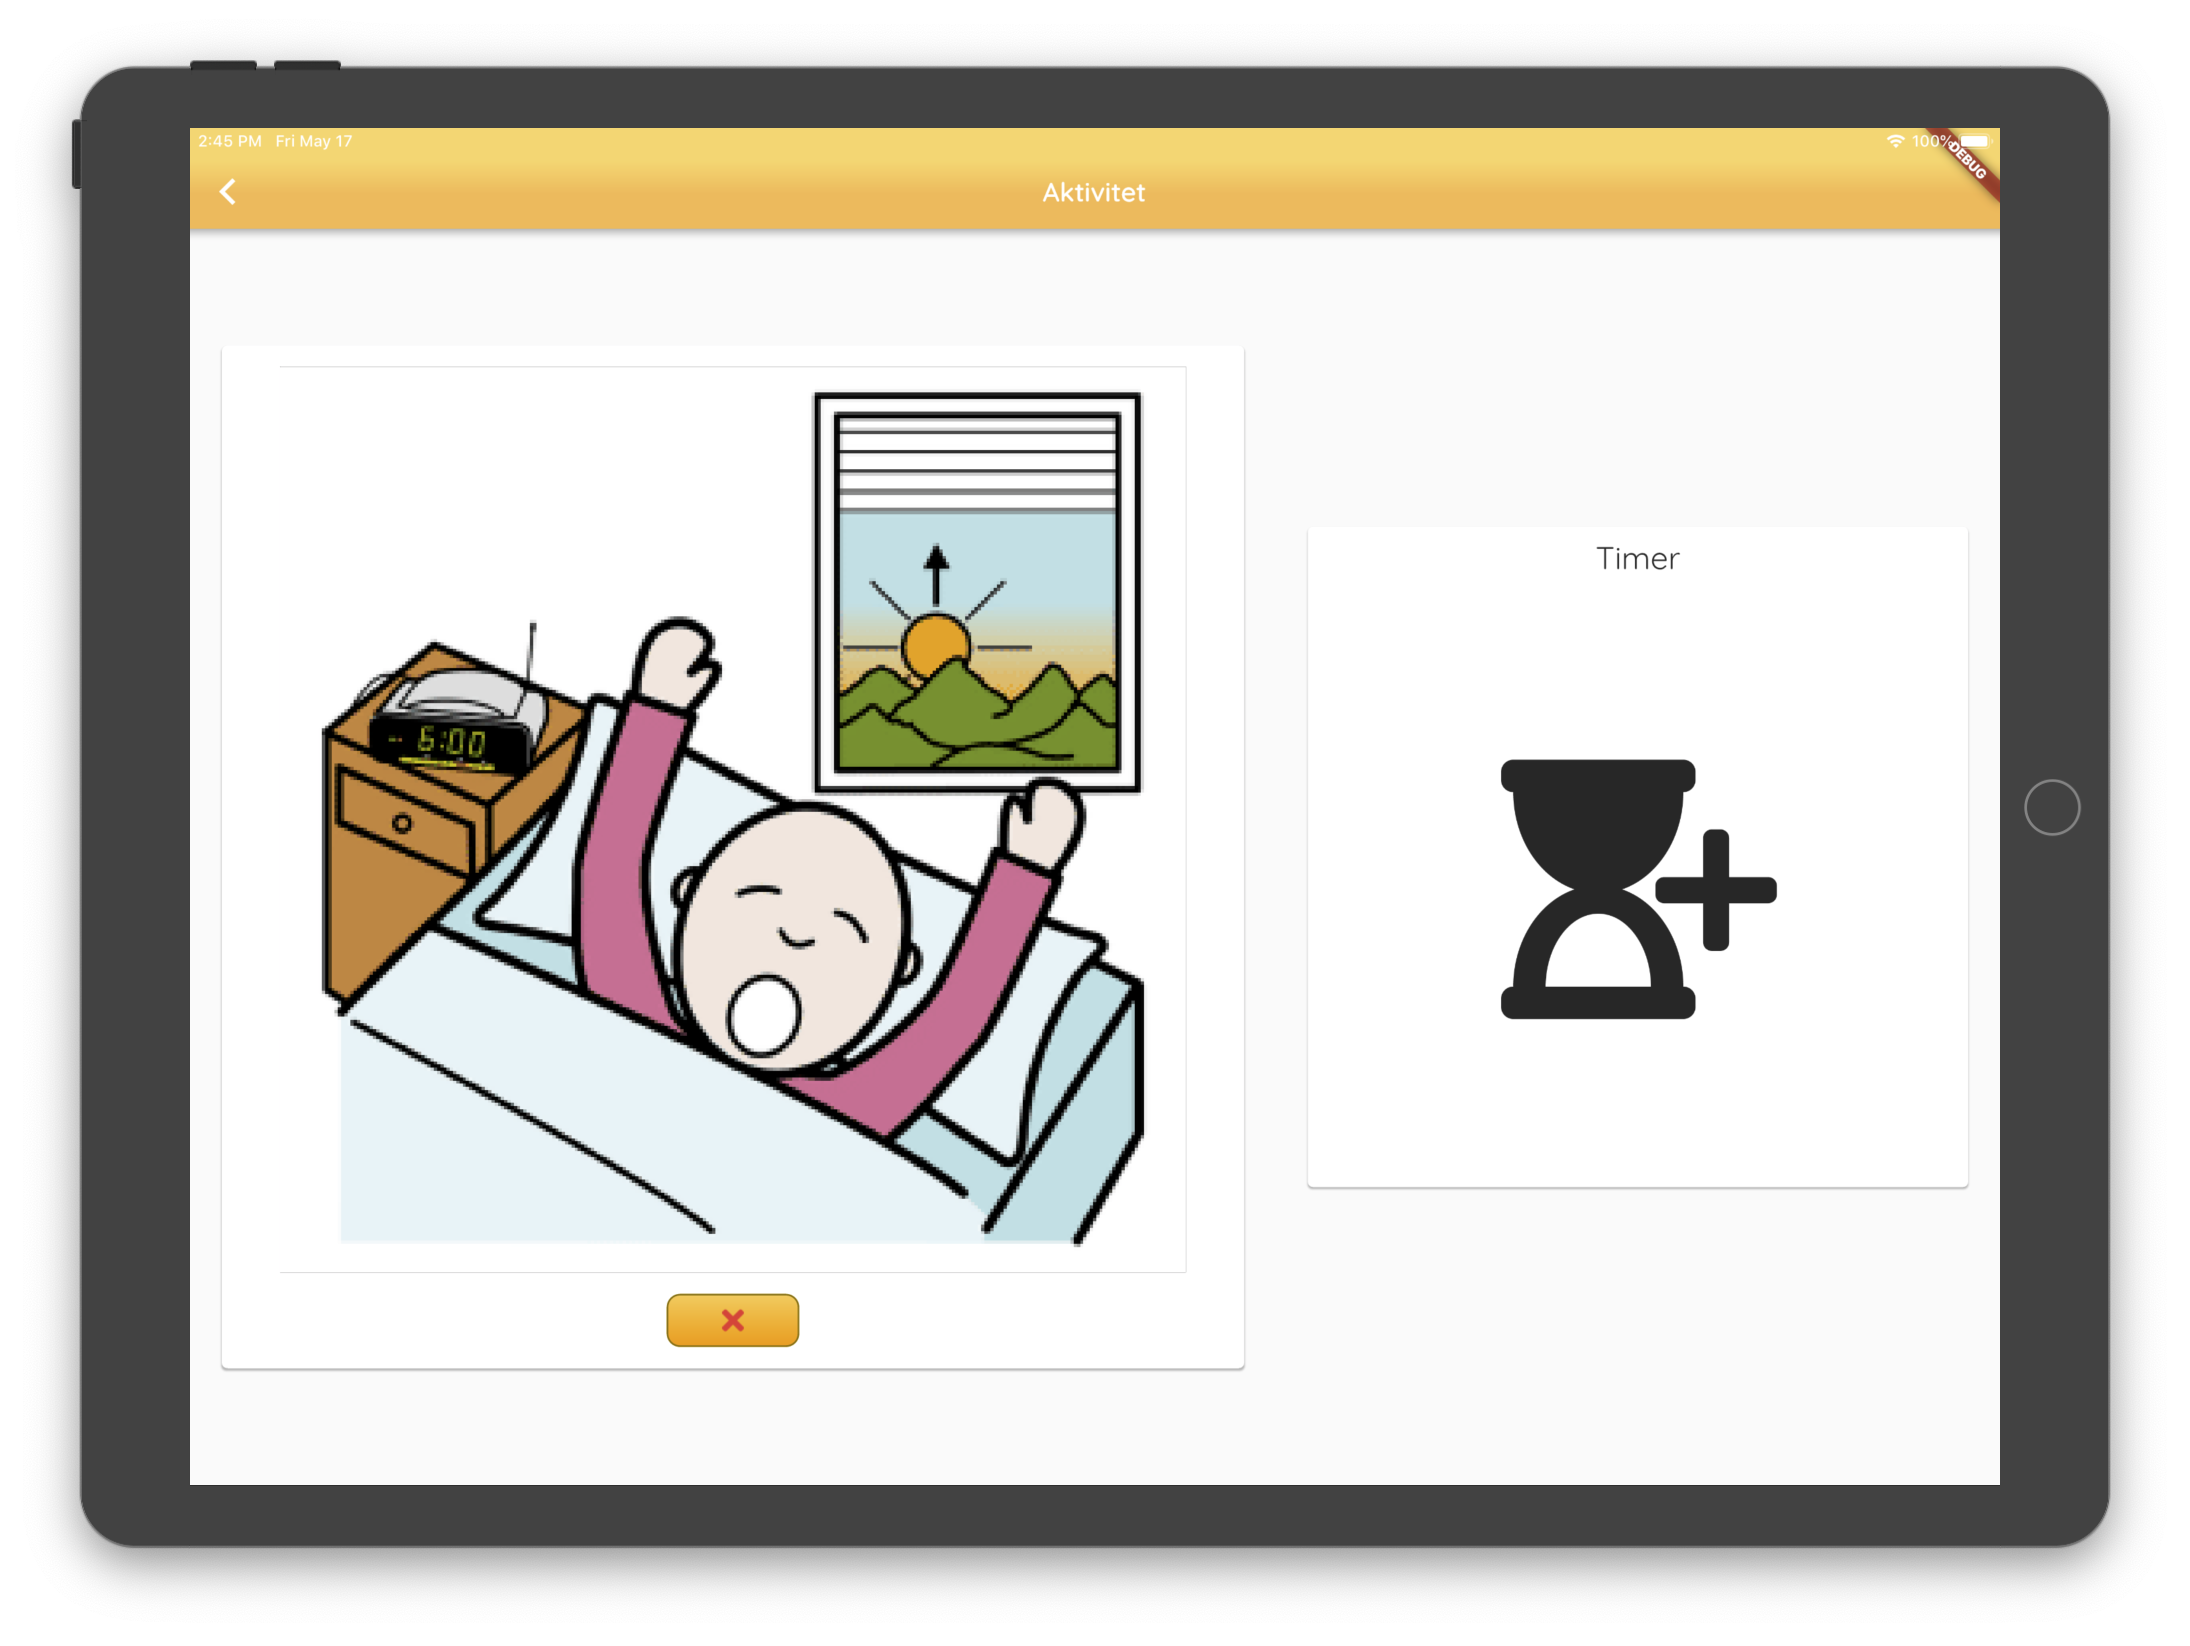
\includegraphics[width=0.95\textwidth]{figures/FinalScreen/showActivityGuardian.png}
    \end{center}
    \caption{Show an activity as guardian without a timer.}
    \label{fig:finalShowActivityGuardianWithoutTimer}
\end{figure}
\begin{figure}[H]
    \begin{center}
        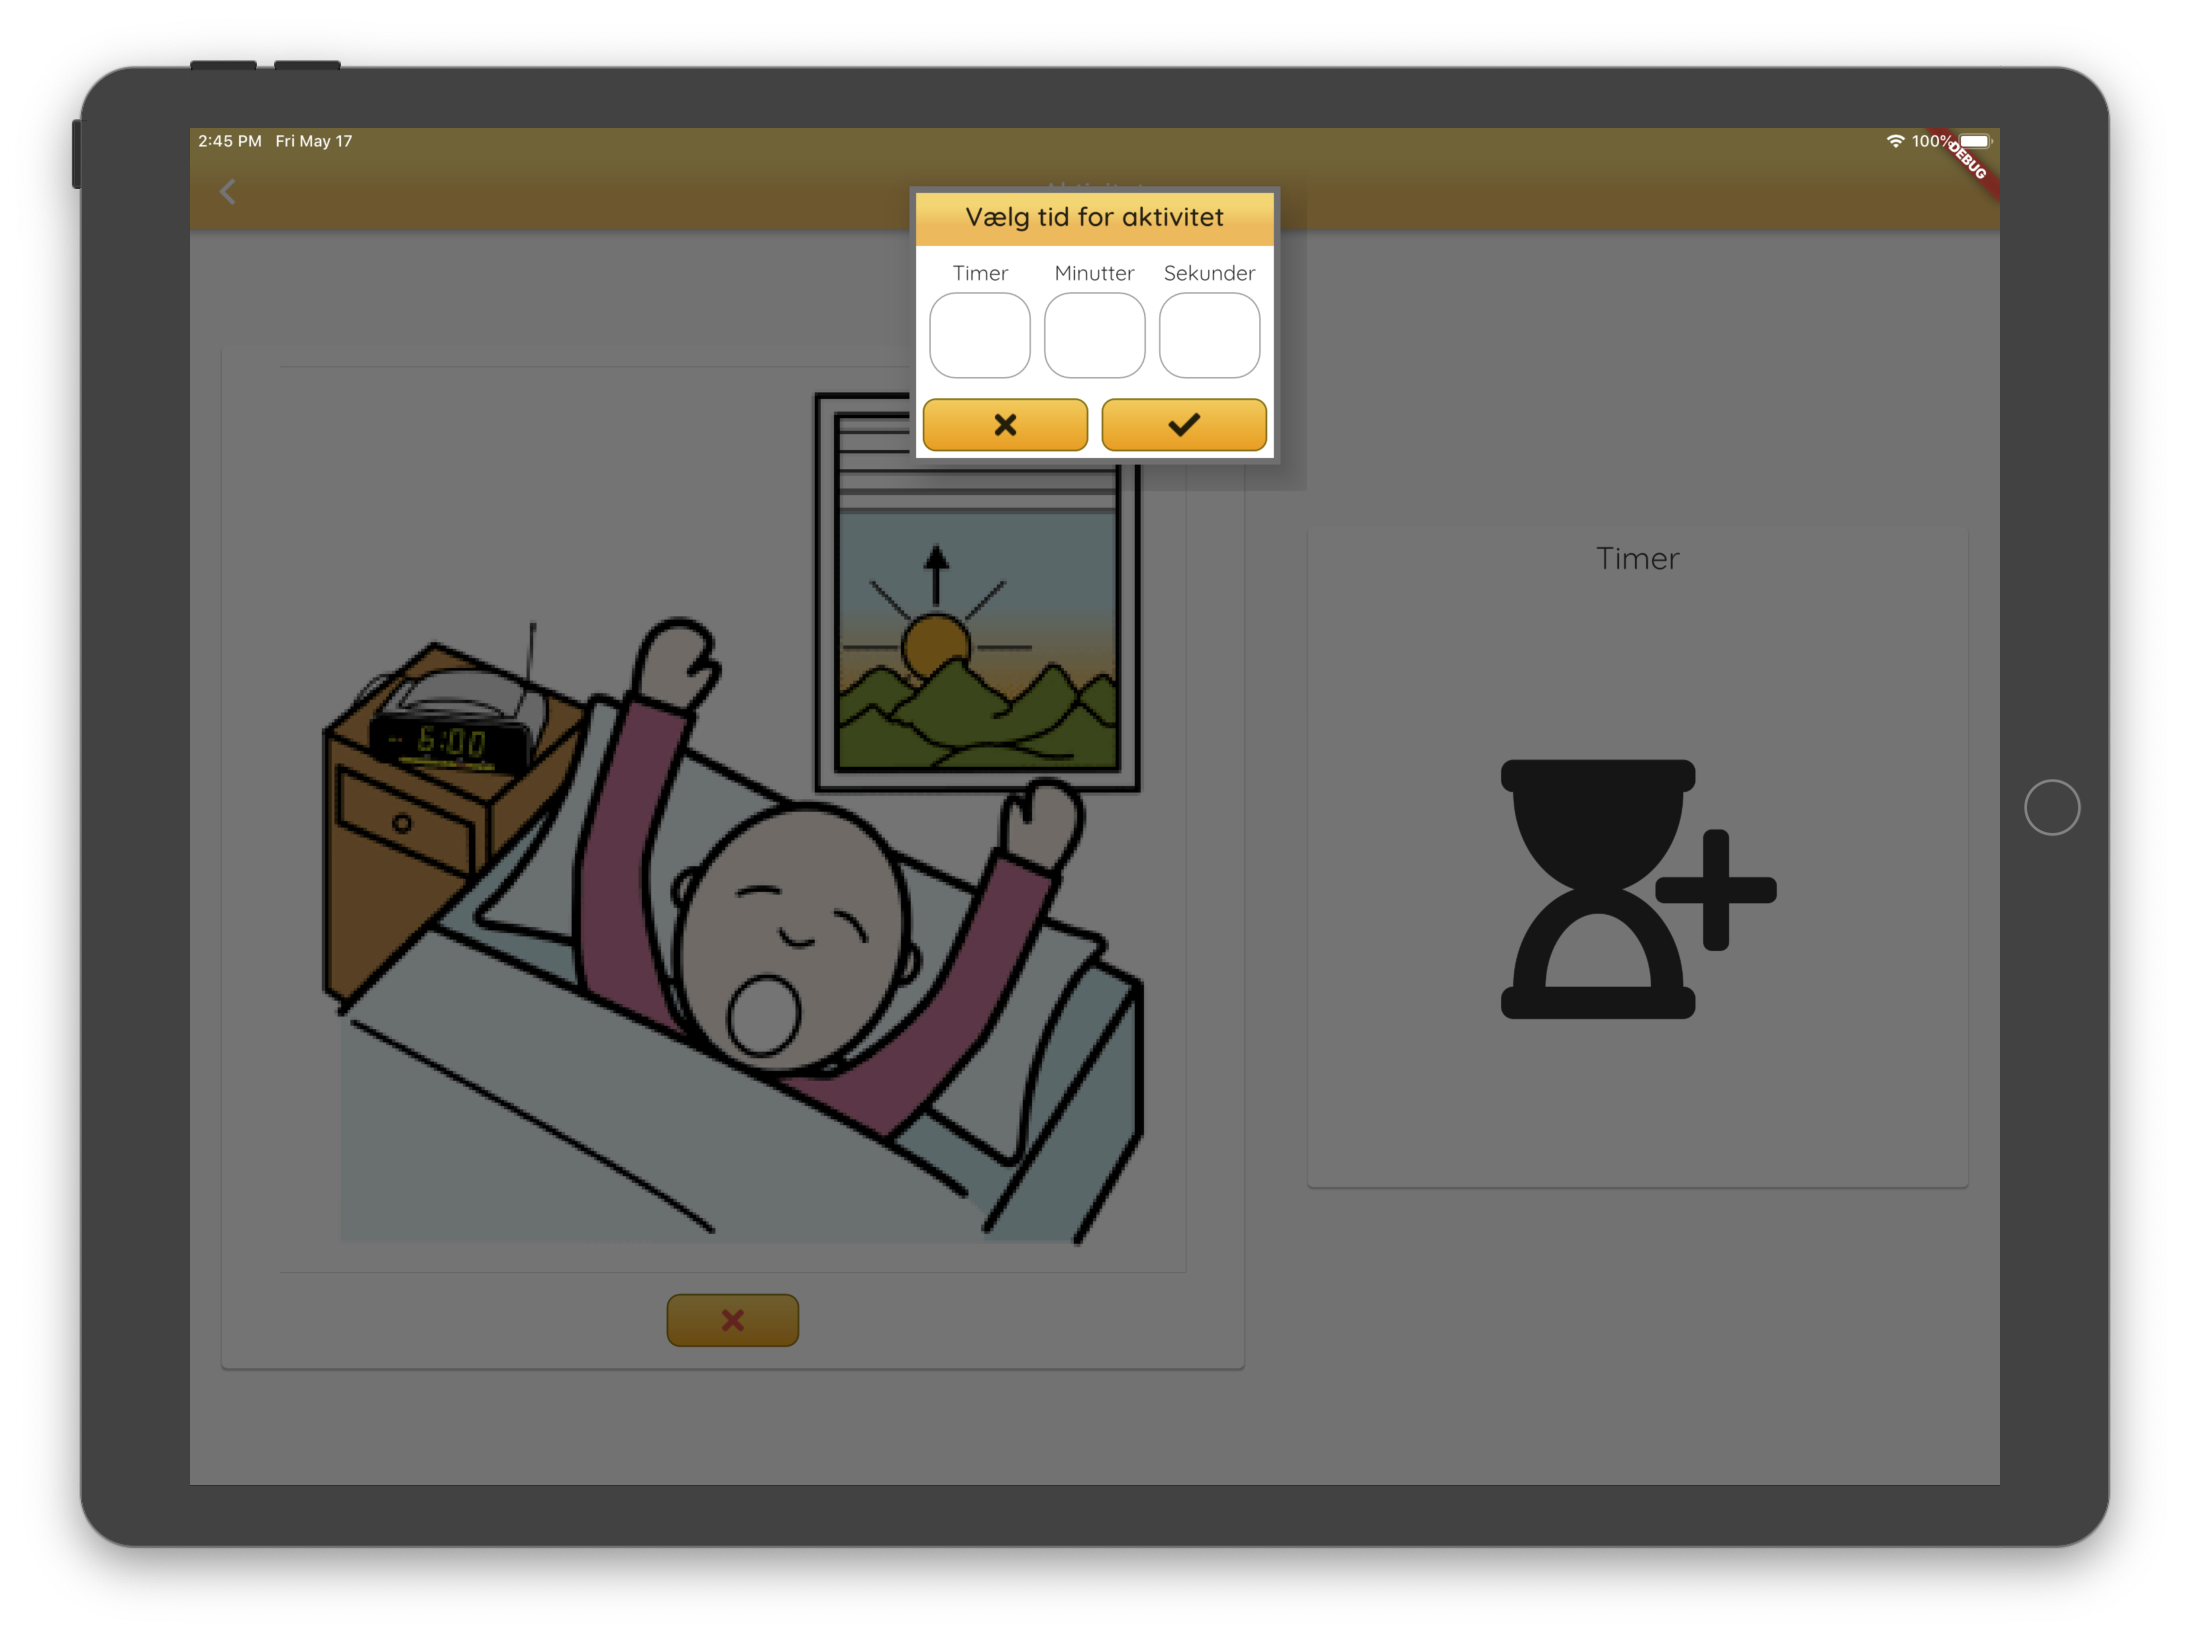
\includegraphics[width=0.95\textwidth]{figures/FinalScreen/showActivityGuardianSetTimer.png}
    \end{center}
    \caption{Set time for activity timer}
    \label{fig:finalShowActivityGuardianSetTimer}
\end{figure}
\begin{figure}[H]
    \begin{center}
        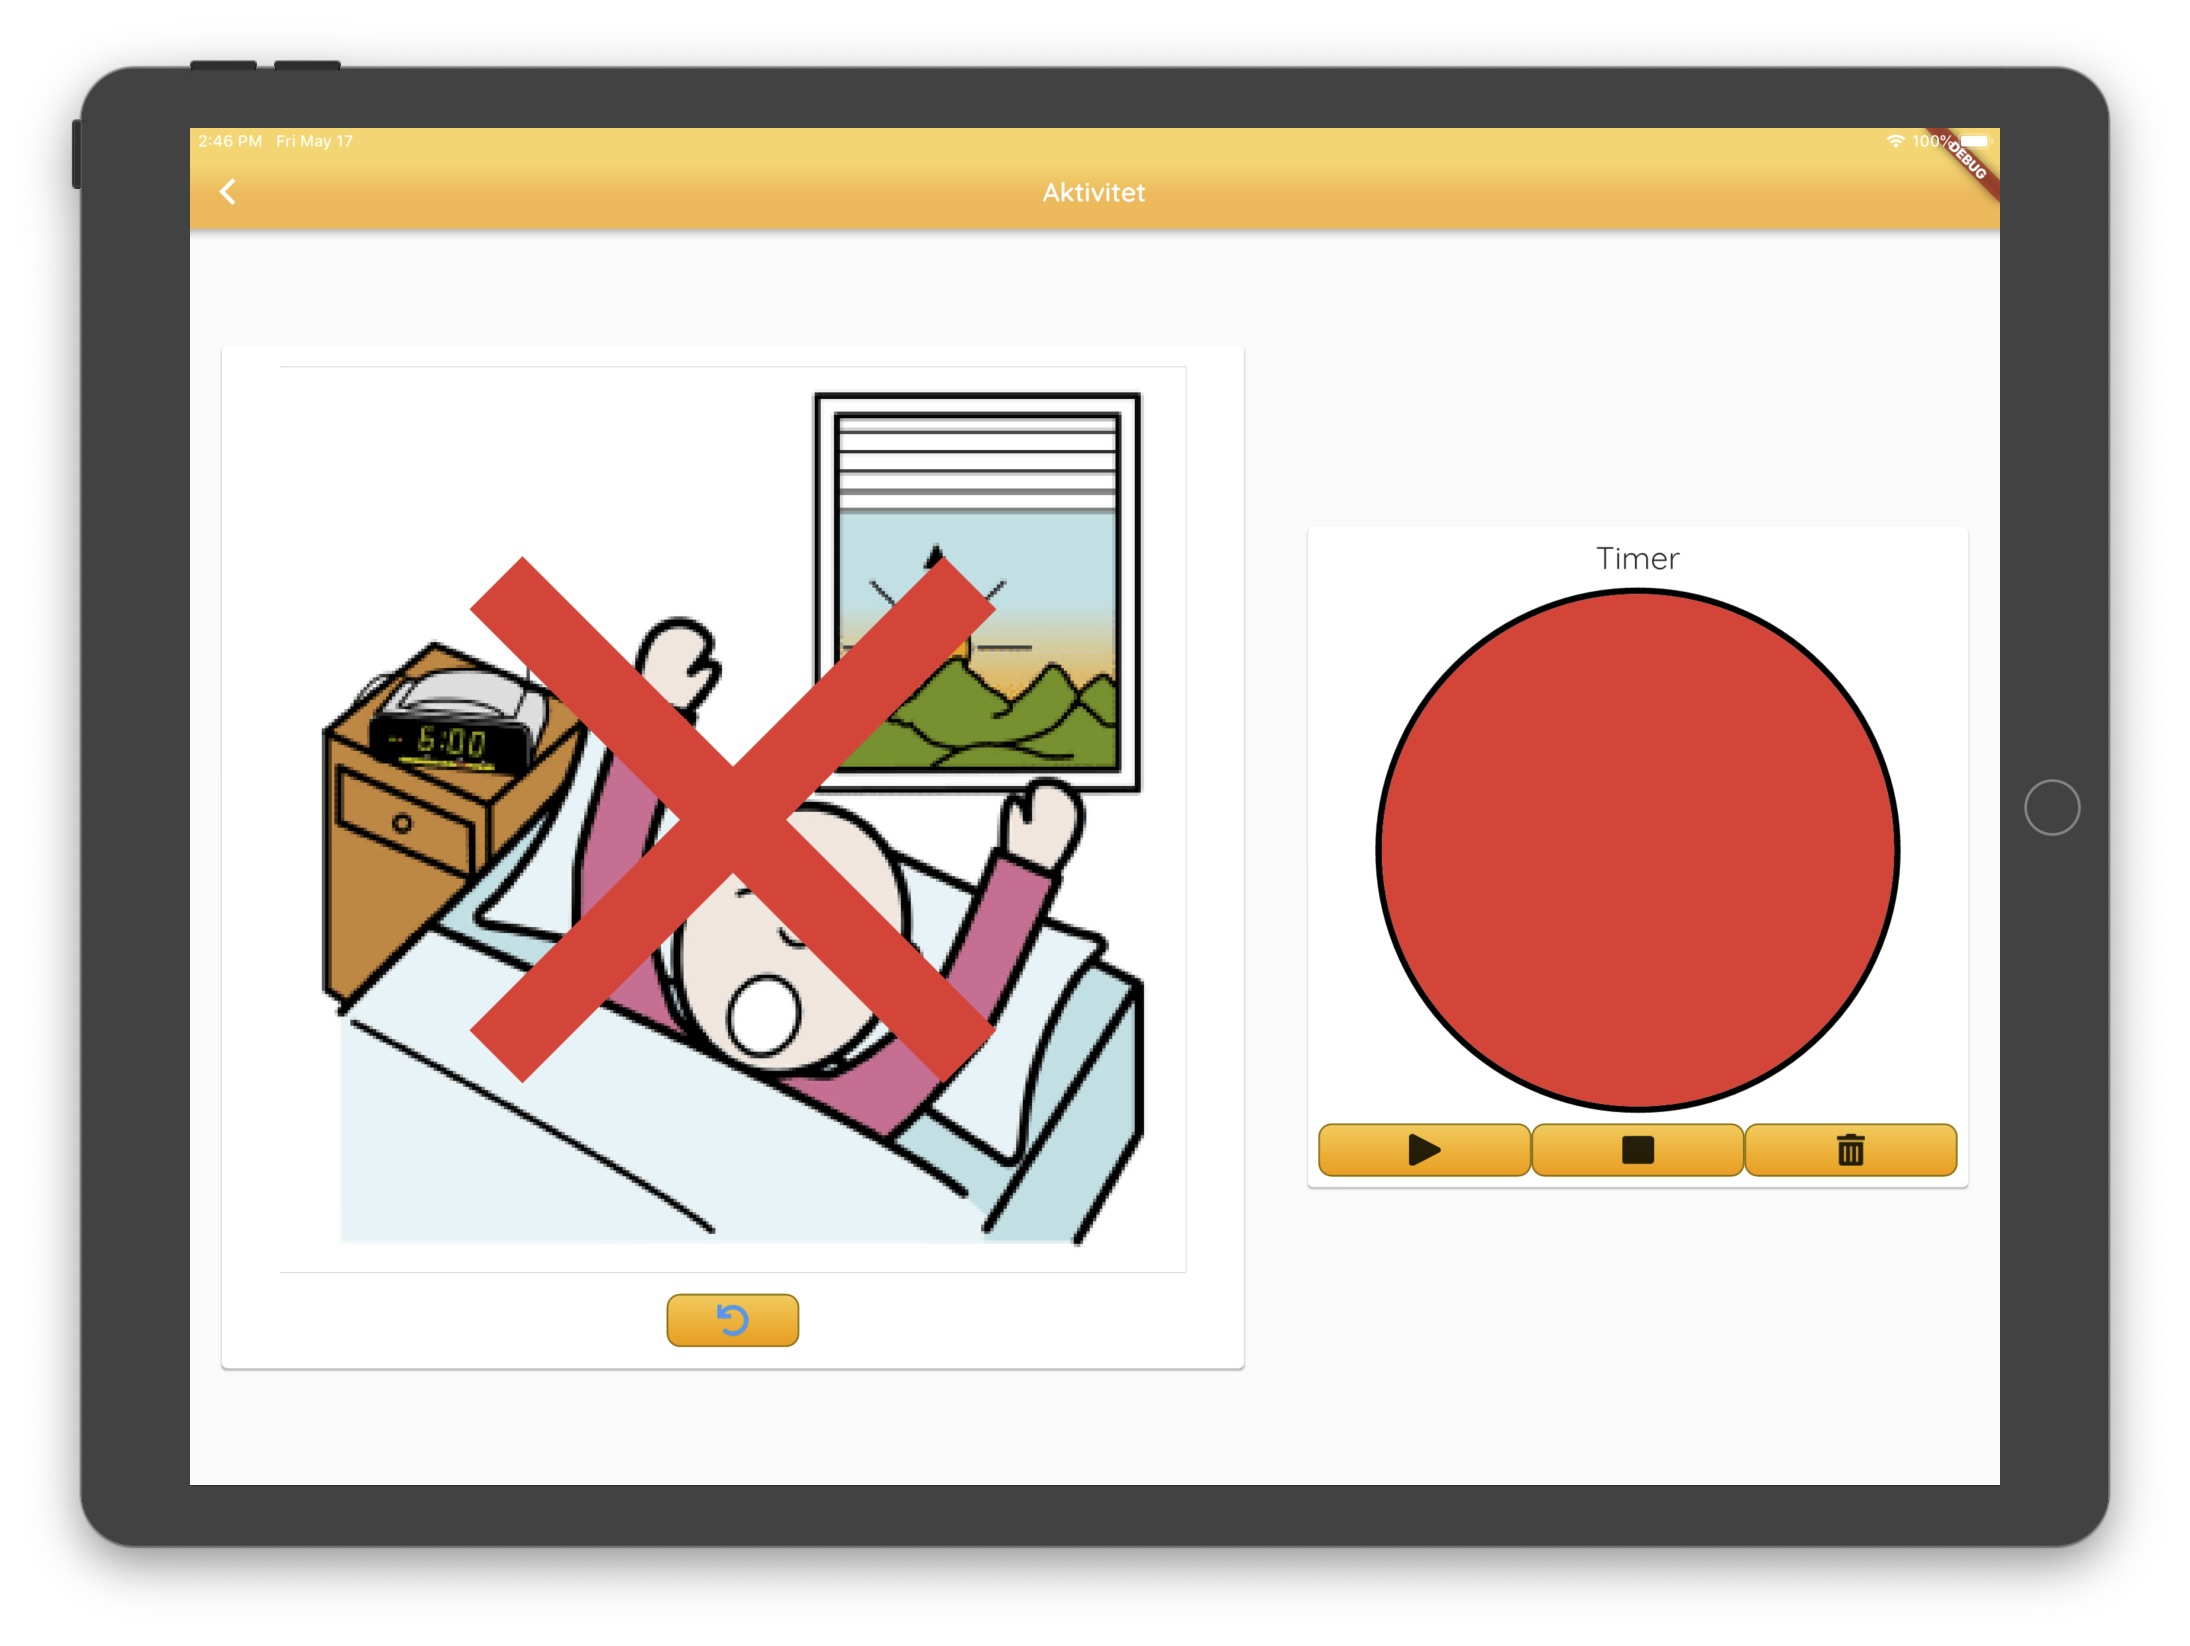
\includegraphics[width=0.95\textwidth]{figures/FinalScreen/showActivityGuardianCanled.png}
    \end{center}
    \caption{Timer set on guardian screen an activity canceled.}
    \label{fig:finalShowActivityGuardianWithTimer}
\end{figure}

\begin{figure}[H]
    \begin{center}
        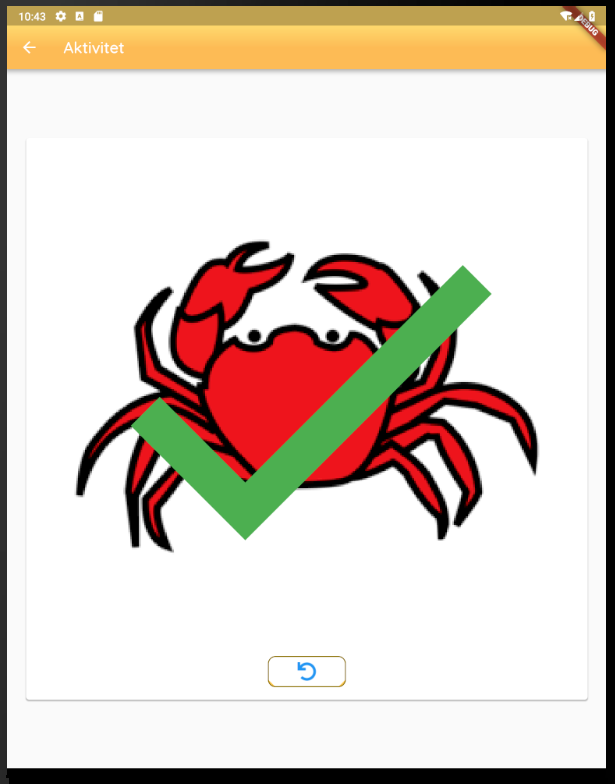
\includegraphics[width=0.95\textwidth]{figures/FinalScreen/showActivityCitizenWithout.png}
    \end{center}
    \caption{Activity screen for citizen mode without timer.}
    \label{fig:finalShowActivityCitizenWithoutTimer}
\end{figure}\begin{figure}[H]
    \begin{center}
        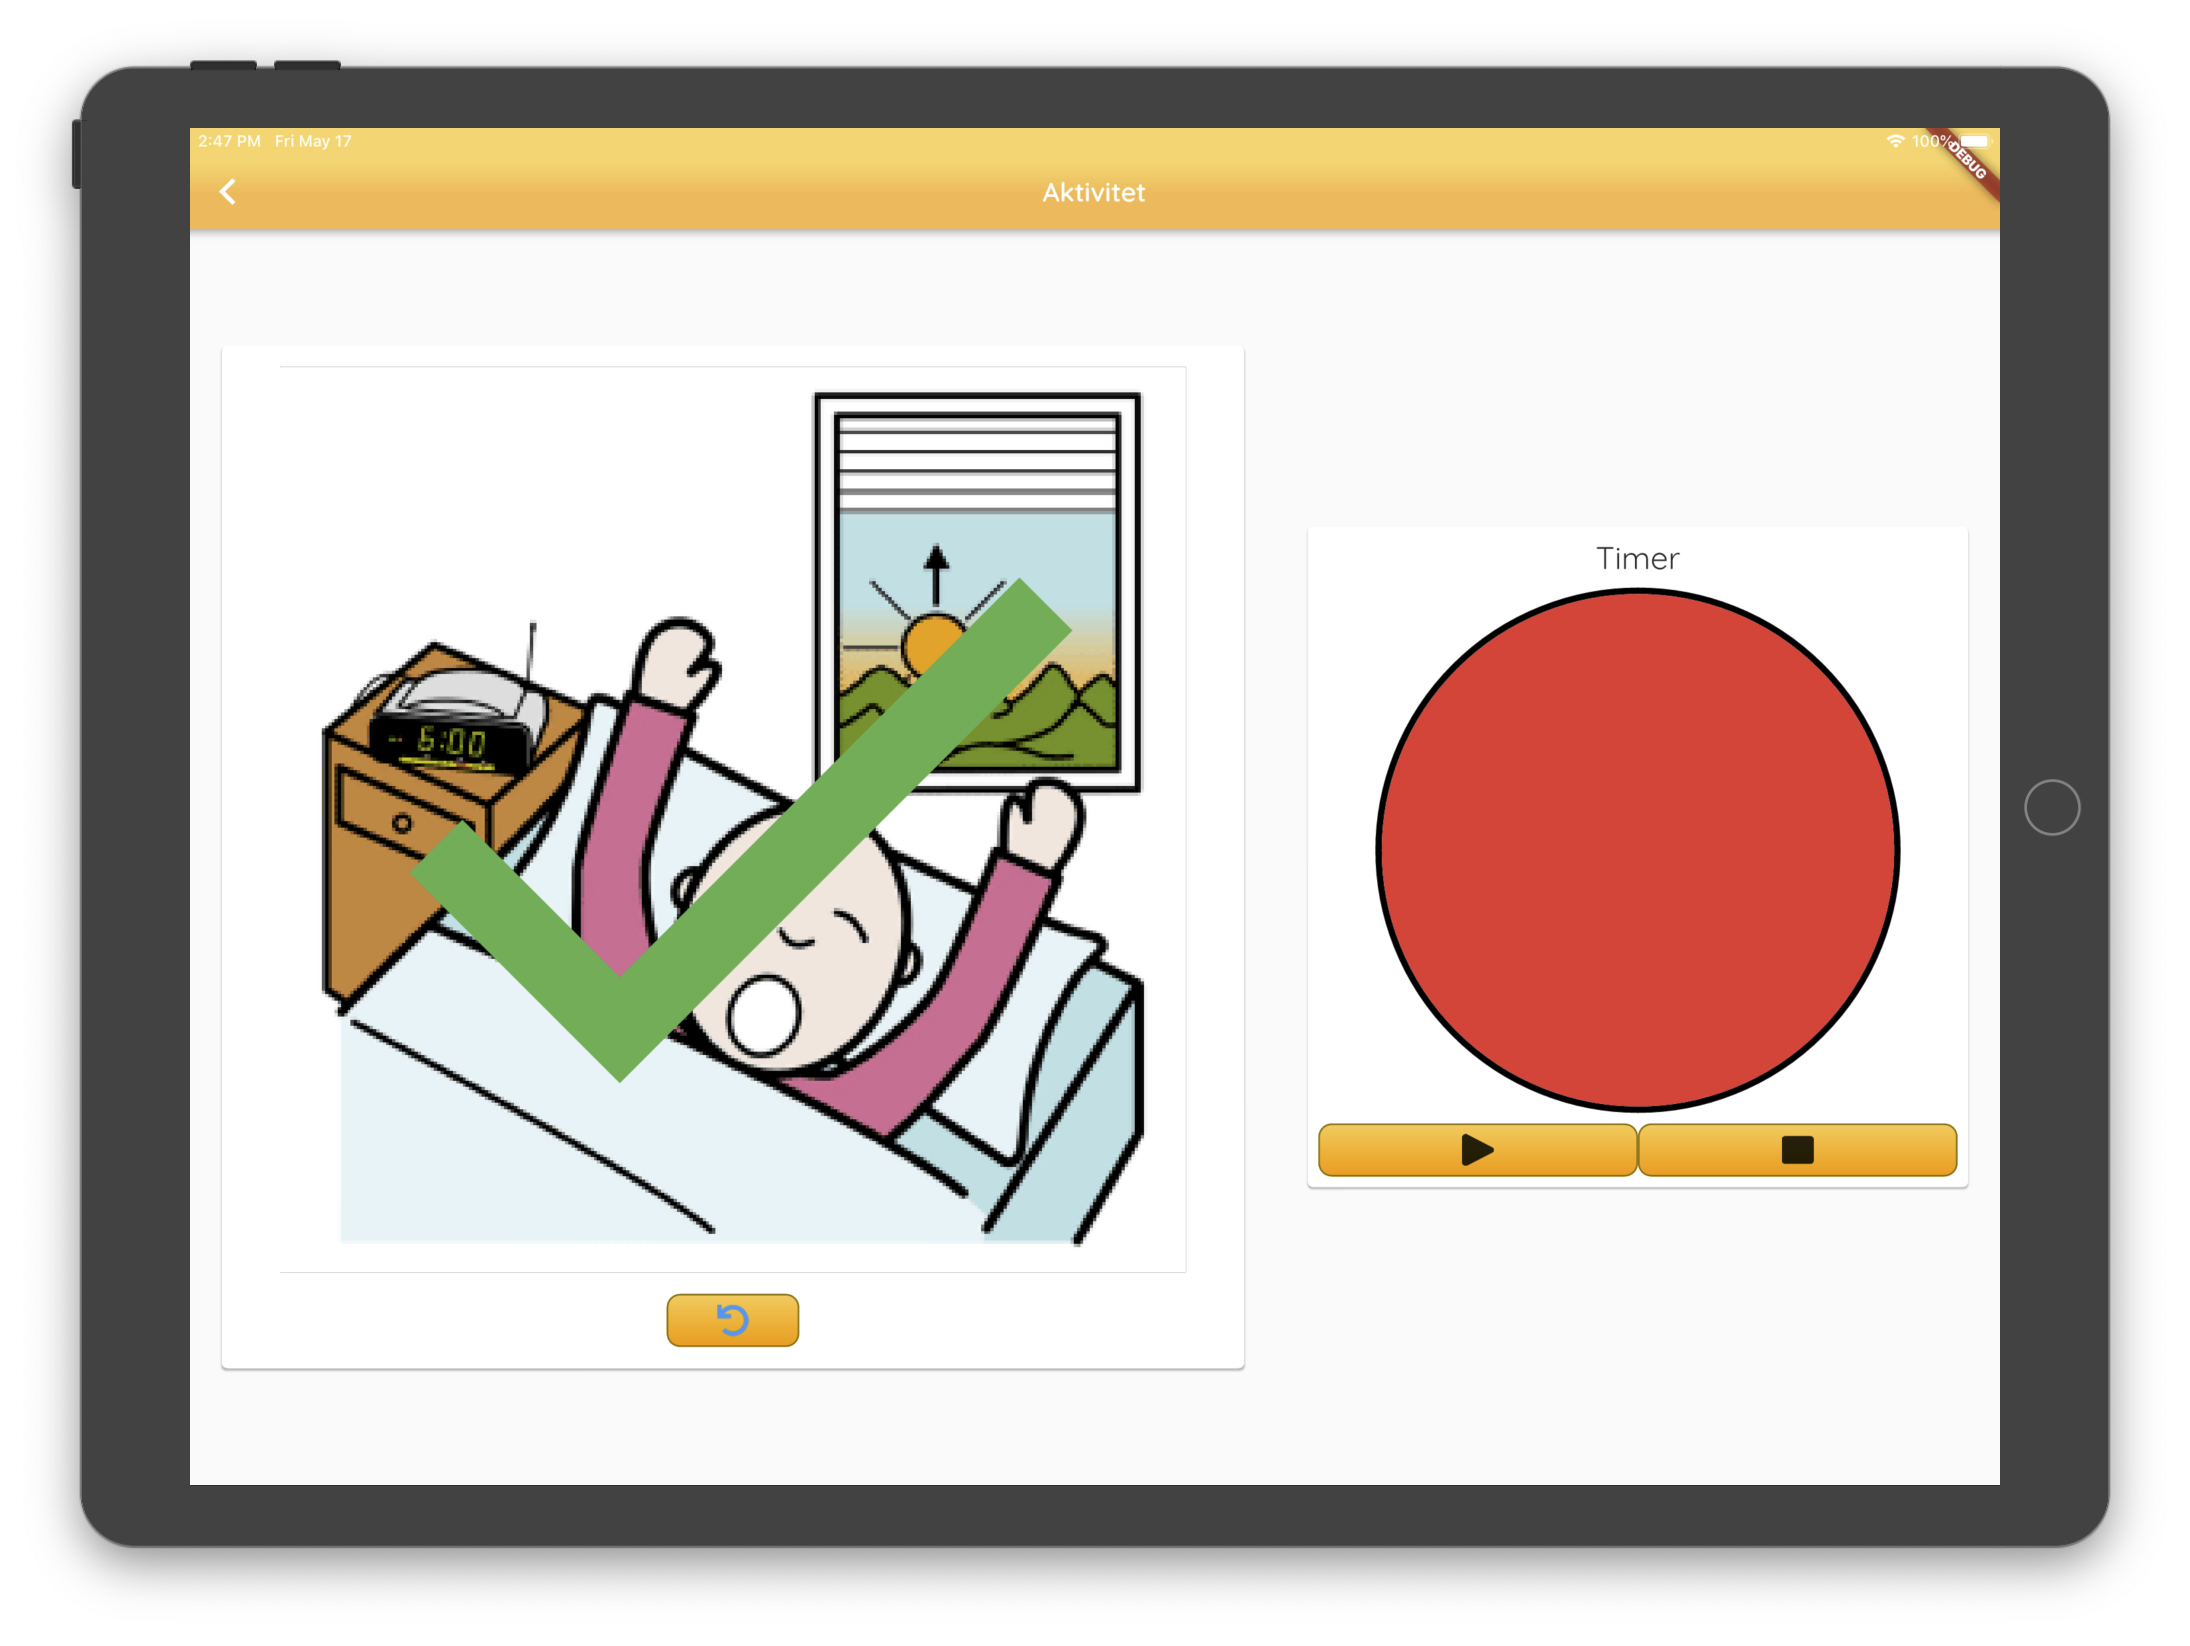
\includegraphics[width=0.95\textwidth]{figures/FinalScreen/showActivityCitizenWithTimer.png}
    \end{center}
    \caption{Activity screen for citizen mode with timer.}
    \label{fig:finalShowActivityCitizenWithTimer}
\end{figure}

In guardian mode an activity can be canceled or uncanceled, or a timer can be set. \ref{fig:finalShowActivityGuardianWithoutTimer} shows the screen before a timer is set. When setting a timer, the duration should be entered in the fields shown in \ref{fig:finalShowActivityGuardianSetTimer}, and a timer appears. \ref{fig:finalShowActivityGuardianWithTimer} shows the screen when a timer is added and the activity is canceled. The timer can be started, paused, stopped or discarded.

The show activity in citizen mode can be seen in \ref{fig:finalShowActivityCitizenWithoutTimer}, where an activity can be marked as done or undone. If a timer is set on the activity, the activity will appear as in \ref{fig:finalShowActivityCitizenWithTimer}. The citizen Can only start, stop and pause a timer. 

\subsection{Upload image from phone screen}

The Upload image from phone screen is shown in \ref{fig:finalUploadPicture}.
\end{figure}\begin{figure}[H]
    \begin{center}
        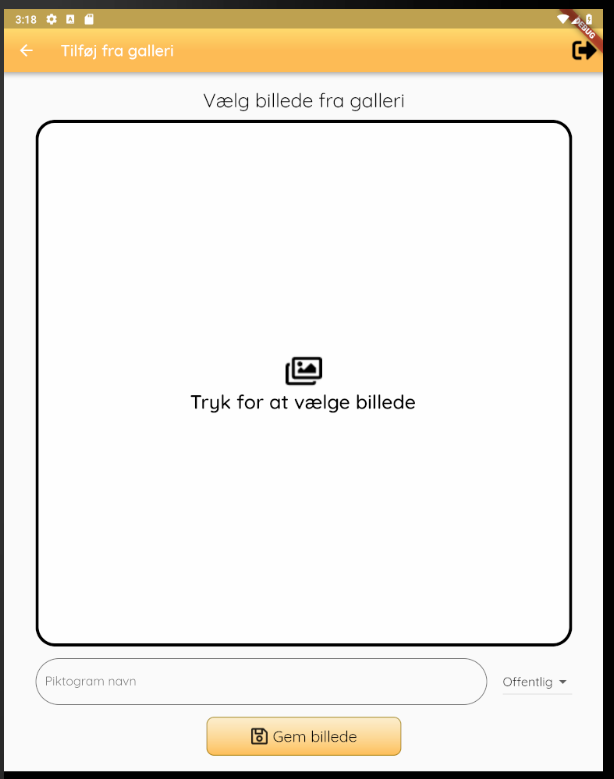
\includegraphics[width=0.95\textwidth]{figures/FinalScreen/addPictogramFromGalleryScreen.png}
    \end{center}
    \caption{The Upload picture from phone screen.}
    \label{fig:finalUploadPicture}
\end{figure}

When the big box is pressed, the phone gallery opens and a picture can be chosen. Before the picture is saved, a pictogram name has to be added in the text box. The option of public or private save is available. The pictogram is added as if it was chosen in the Choose pictogram screen, and saved in the database. 

These are the main features and functionalities of the weekplanner application.